\documentclass{moncours}
\usepackage{float}
\makeindex




\begin{document}

\newcounter{tmp} % pour couper les boîtes énoncés au milieu d'un enumerate

\renewcommand{\labelitemi}{\textbullet}
\renewcommand{\labelitemii}{$\circ$} 

\frontmatter

\titlePage[./images/couvertureFlo5e_v11]{Informatique 5\up{e}}{Fiches MITIC}{Institut Florimont}{\textcopyright\ Tout droit réservé. Crédit photographie couverture : Institut Florimont. Illustration des premières pages de chapitre issue de \emph{Codex Leicester} de Leonardo da Vinci (domaine public).  \\ Version : janvier 2021 \\ 2\up{ème} édition, v1.1 \\ Petit-Lancy (Suisse)} 

% TOC
\pagestyle{empty} % No headers

\tableofcontents % Print the table of contents itself
\cleardoublepage % Forces the first chapter to start on an odd page so it's on the right
\pagestyle{fancy} % Print headers again

\cleardoublepage % on force une page impaire
\vspace*{1cm}

\section*{Calendrier des différentes activités (5\up{e})}\index{Calendrier des activités}  

\vfill

\begingroup % permet de bloquer le arraystretch à ce groupe seulement
\renewcommand{\arraystretch}{1.2}
\begin{center}
\begin{tabular}{|l|l|c|l|l|}
\hline
\multirow{2}{*}{\textbf{Nom de la fiche}} & \multirow{2}{*}{\textbf{Matière}} & \multirow{2}{*}{\textbf{Page}} & \textbf{Date de} & \textbf{Nom du} \\
 &  &  & \textbf{réalisation} & \textbf{professeur} \\ \hline
%\rowcolor[gray]{0.8}\multicolumn{5}{|l|}{Rentrée scolaire} \\ \hline 
%\emph{La plateforme Flore} & (Titulaire) & \pageref{plateformeFlore} & & \phantom{xxxxxxxxxxxxxxxx}  \\ \hline
%
% avant les vacances d'octobre
%
\rowcolor[gray]{0.8}\multicolumn{5}{|l|}{Avant les vacances d'octobre} \\ \hline
\emph{Tableur : séance 1} & Physique-Chimie & \pageref{ficheTableur5e1} & & \\ \hline
\emph{Texte : séance 1} & Français & \pageref{ficheTexte5e1} & & \\ \hline \hline
%
% avant les vacances de Noël
%
\rowcolor[gray]{0.8}\multicolumn{5}{|l|}{Avant les vacances de Noël} \\ \hline
\emph{Tableur : séance 2} & Mathématiques & \pageref{ficheTableur5e2} & & \\ \hline

\emph{Scratch : séance 1} & Mathématiques & \pageref{ficheScratch5e1} & & \\ \hline \hline
%
% avant les vacances de février
%
%\rowcolor[gray]{0.8}\multicolumn{5}{|l|}{Avant les vacances de février} \\ \hline
%
% avant les vacances de printemps
%
\rowcolor[gray]{0.8}\multicolumn{5}{|l|}{Avant les vacances de printemps} \\ \hline
\emph{Texte : séance 2} & Anglais & \pageref{ficheTexte5e2} & & \\ \hline
\emph{Scratch : séance 2} & Mathématiques & \pageref{ficheScratch5e2} & & \\ \hline
\emph{Son : séance 1} & Anglais & \pageref{ficheSon5e1} & & \\ \hline \hline
%
% avant les vacances d'été
%
\rowcolor[gray]{0.8}\multicolumn{5}{|l|}{Avant les vacances d'été} \\ \hline
\emph{Image : séance 1} & Français & \pageref{ficheImage5e1} & & \\ \hline
\emph{Scratch : séance 3} & Mathématiques & \pageref{ficheScratch5e3} & & \\ \hline \hline
%
% avant la fin du semestre de cours
%
\rowcolor[gray]{0.8}\multicolumn{5}{|l|}{Avant la fin du semestre de cours (pour les cours au semestre)} \\ \hline
\emph{Tableur : séance 3} & Géographie & \pageref{ficheTableur5e3} & & \\ \hline
\emph{Texte : séance 3} & Histoire & \pageref{ficheTexte5e3} & & \\ \hline
\emph{Image : séance 2} & Arts visuels & \pageref{ficheImage5e2} & & \\ \hline
%\emph{Son : séance 2} & Musique & \pageref{ficheSon5e2} & & \\ \hline
\end{tabular}
\end{center}
\endgroup

\vfill

\cleardoublepage % on force une page impaire pour le clavier
\section*{Les touches spéciales du clavier}\index{Clavier}\index{Touches spéciales}

\vfill

\begin{center}
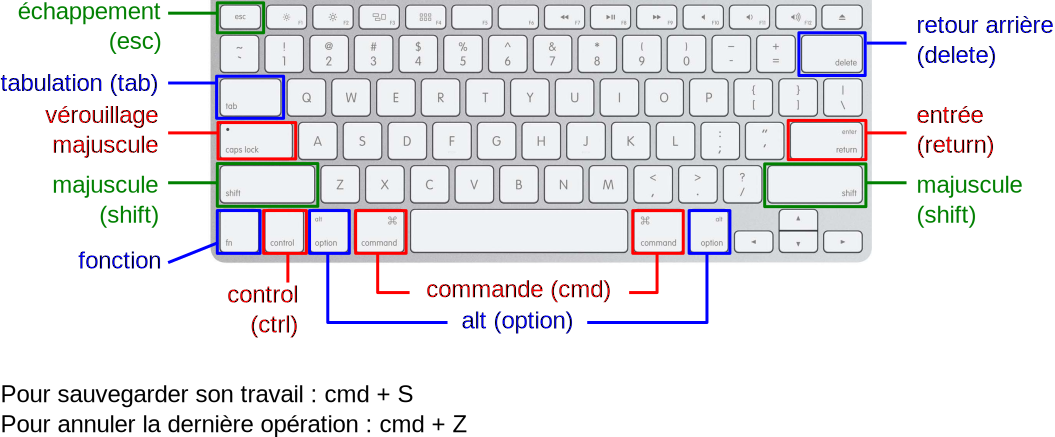
\includegraphics[angle=90,width=.6\textwidth]{./images/generales/clavierTouches}
\end{center}

\vfill

\cleardoublepage % on force une page impaire pour la philosophie du document
\chapter*{Philosophie du document}


\prof{\textbf{ceci est la version professeur du document.} L'icône du professeur est suivie par des informations complémentaires qui n'apparaissent pas dans la version élève.}  

Vous avez entre les mains le deuxième tome d'une série de trois fascicules qui accompagneront les élèves des classes de 6\up{e}, 5\up{e} et 4\up{e} jusqu'au moment où ils recevront un ordinateur qu'ils seront en mesure d'exploiter au mieux pour leur travail.

\vspace{18pt}

Ce document se présente sous la forme d'un livret qui rassemble des fiches MITIC\footnote{MITIC : Médias, Images et Technologies de l'Information et de la Communication.} permettant aux élèves d'apprendre à utiliser les logiciels et espaces numériques mis à leur disposition. Pour l'année de 5\up{e}, sont traités les logiciels \emph{Microsoft Word} (traitement de texte), \emph{Microsoft Excel} (tableur grapheur), \emph{Gimp} (retouche d'image), \emph{Audacity} (traitement des fichiers son) et \emph{Scratch} (programmation). Au début de chaque chapitre un lien permettant de télécharger le logiciel est fourni.

\vspace{18pt}


Chaque fiche est conçue pour être exploitée à plusieurs occasions et dans des matières différentes, à chaque fois lors d'une séance de 45 minutes. La fiche sur le tableur, par exemple, est découverte en physique-chimie (\emph{Séance 1}), exploitée à nouveau en mathématiques (\emph{Séance 2}) puis en histoire-géographie (\emph{Séance 3}) selon un calendrier proposé en début de fiche. Nous avons à chaque fois essayé de faire coïncider les notions abordées dans la fiche avec le programme de la matière concernée.

\vspace{18pt}
\prof{
Professeurs, c'est à vous que revient la tâche délicate d'inclure le contenu de ces fiches dans votre progression. À vous de le faire vivre : arriver en salle informatique et demander aux élèves de remettre en forme un texte de Molière ne présente que peu d'intérêt pédagogique. Donnez du sens à ces fiches et profitez-en pour diversifier votre enseignement. N'hésitez pas à exploiter dans vos cours les techniques présentées dans ce fascicule afin que les élèves utilisent plusieurs fois leurs nouvelles compétences et, par là-même, les pérennisent.
}
%\vspace{18pt}

%Ces fiches MITIC sont appelées à évoluer. N'hésitez pas à nous transmettre vos suggestions et nous signaler toute erreur relevée par courriel à l'adresse \texttt{flo-mitic@florimont.ch}.

%\vspace{18pt}

Merci d'avance à tous pour votre implication.

\vspace{18pt}

L'équipe de rédaction.

\vspace{2cm}

% \emph{Remarque : il existe une version professeur de ce document, contenant des informations complémentaires, disponible sur l'ENT de l'école.}

  


% Début des chapitres
%\setcounter{page}{1} % si on veut forcer la page 1 au début du premier chapitre
\mainmatter
%
  
\chapterImage{./images/chapitreVinci5e}
\chapter{Annexe - Microsoft Teams}\label{teams1}  


La suite Microsoft comporte plusieurs applications qui possèdent des fonctionnalités différentes. En particulier, on notera les applications suivantes :\\

\begin{itemize}
\item \textit{Word} - est un éditeur de traitement de texte.
\item \textit{Excel} - est un tableur offrant une organisation visuelle des données et des outils d'analyse de contenu.
\item \textit{PowerPoint} - permet de créer des présentations.
\item \textit{Outlook} - est un outil de gestion des e-mails proposant un calendrier.
\item \textit{OneNote} - est un éditeur de prises de notes.
\item \textit{OneDrive} - est un cloud permettant de stocker des données sur des serveurs distants.
\item \textit{Teams} - est un outil centralisé permettant le travail collaboratif. Il gère notamment l'accès à OneNote, OneDrive ainsi qu'à la messagerie instantanée et Ourlook.
%\item \textit{Access} - est un gestionnaire de bases de données permettant la création d'applications commerciales.
%\item \textit{Edge} - est un navigator permettant l'accès à Internet.
%\item \textit{Skype} - est un gestionnaire de communication pour les appels et le chat.
%\item \textit{Sway} - est un outil de création de rapports et de newsletters interactives.
\end{itemize} 


% CONNEXION A OFFICE
\section{Connexion à Office 365 et Teams}

Ouvrez le navigateur internet de votre choix ou Safari et entrez l'URL suivante: \url{www.office.com}. Cliquez sur \textit{Connexion}.

\begin{figure}[H]
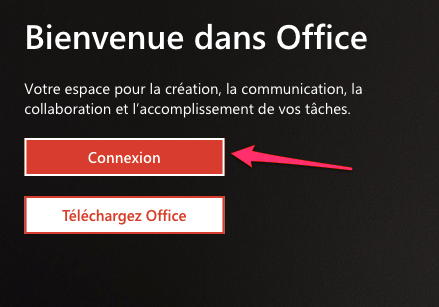
\includegraphics[width=5cm]{./images/teams/ecran_office_com_crop}
\centering
\end{figure}

Vous arrivez sur l'écran de connexion de microsoft office en ligne. Entrez votre adresse mail de l'école (qui se termine donc par \textit{@florimont.ch}).

\begin{figure}[H]
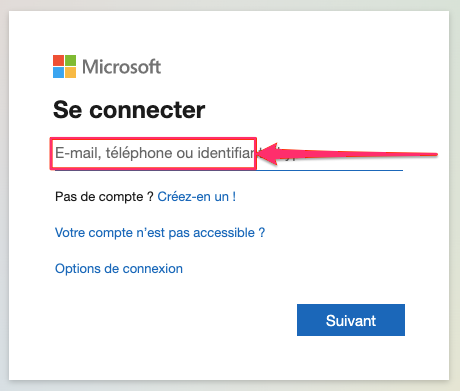
\includegraphics[width=5cm]{./images/teams/ecran_connexion_office_com_crop}
\centering
\end{figure}

Vous êtes alors redirigé vers la page d'identification de l’école. Entrez votre mot de passe. (l'adresse mail est déjà entrée, mais vous pouvez la modifier au cas où vous avez fait une erreur lors de l'étape précédente.)

\begin{figure}[H]
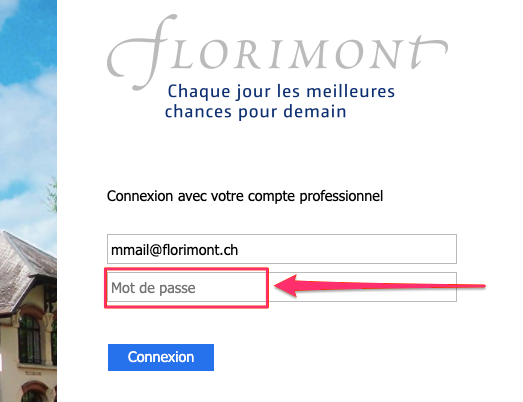
\includegraphics[width=5cm]{./images/teams/ecran_connexion_florimont_crop}
\centering
\end{figure}

Il se peut qu'on vous demande si vous voulez rester connecté. Si vous comptez travailler longtemps sur cette session, il vaut mieux accepter.\\

En revanche, si le navigateur vous propose d'enregistrer votre mot de passe, il est recommandé de refuser (soit en fermant la fenêtre, soit en choisissant \textit{Jamais}). Si vous vous connectez depuis votre ordinateur personnel, il peut être pratique de permettre au navigateur de se souvenir de mots de passe, mais ce n'est jamais une bonne idée sur un ordinateur partagé ou d'emprunt.\\

Le site vous proposera peut-être de télécharger l’application. Cliquez alors sur \textit{Utiliser l’application web à la place}.\\

Alternativement, sur certains navigateurs (comme Safari), vous devrez télécharger l'application de bureau Teams. Cliquez sur \textit{Télécharger l'application} pour continuer.

\begin{figure}[H]
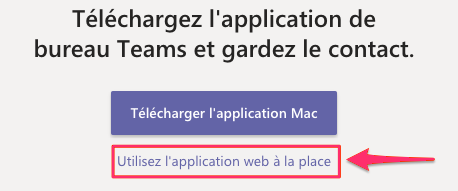
\includegraphics[width=6cm]{./images/teams/ecran_installer_teams_crop}
\centering
\end{figure}

Vous arrivez sur la page de téléchargement de l'application. Cliquez sur \textit{Download Teams}, sous le logo de la pomme, pour télécharger l'application pour Mac.\\

Vous êtes à présent dans votre espace Office. Sur la gauche, choisissez l'icône Teams.

\begin{figure}[H]
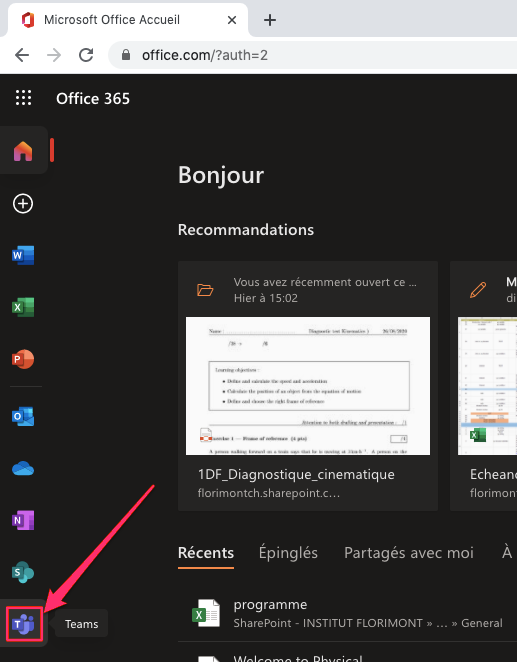
\includegraphics[width=5cm]{./images/teams/ecran_accueil_office_crop}
\centering
\end{figure}

Félicitations, vous arrivez sur la page d'accueil de votre session Teams.




% UTILISATION DE LA PUBLICATION
\section{Utilisation de la Publication}

La messagerie instantanée proposée pour chaque équipe doit permettre aux élèves et aux enseignants de communiquer en dehors de l'école dans un cadre qui reste strictement scolaire. Ainsi les messages personnels n'ont aucune raison d'être sur Teams. Il vous appartient donc de mesurer vos propos lorsque vous utilisez la messagerie instantanée. Ainsi, toute forme d'insulte ou de critique envers un membre de la classe ou une personne extérieure est à proscrire. Le modérateur de chaque équipe est son enseignant responsable.\\

Pour utiliser la messagerie, il suffit de vous rendre sur l'onglet \textit{Publications}

\begin{figure}[H]
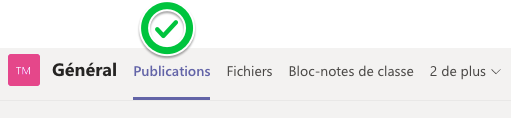
\includegraphics[width=9cm]{./images/teams/publications}
\centering
\end{figure}

puis de rédiger du texte à l'intérieur du champ \textit{Démarrer une conversation}. Utilisez @ pour mentionner un contact, ce qui signifie qu'une notification sera adressée à cette personne. Attention donc de ne pas mentionner un contact inutilement.

\begin{figure}[H]
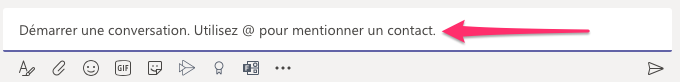
\includegraphics[width=9cm]{./images/teams/publications2}
\centering
\end{figure}

Il ne vous reste plus qu'à cliquer sur l'icône 
\includegraphics[width=0.7cm]{./images/teams/envoi_message} pour envoyer votre message.

\begin{figure}[H]
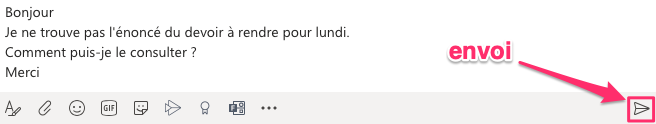
\includegraphics[width=9cm]{./images/teams/publications3}
\centering
\end{figure}





% CONSULTER ET TELECHARGER UN DOCUMENT
\section{Consulter et télécharger un document}

Vous devrez souvent chercher des documents mis en ligne par vos enseignants. Pour faire cela, sélectionnez l'onglet Fichiers, en haut.

\begin{figure}[H]
	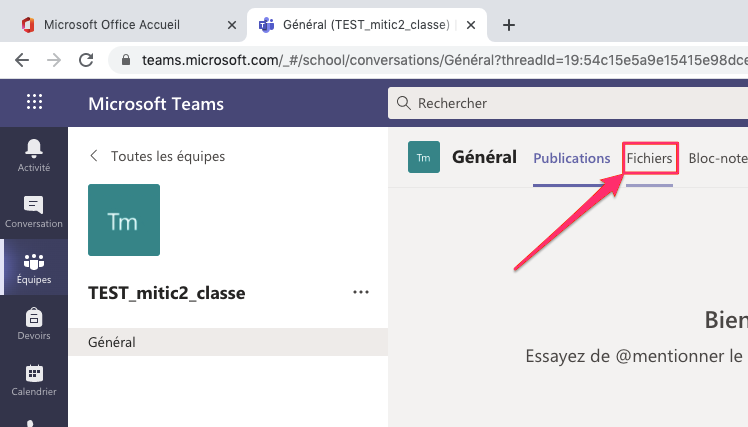
\includegraphics[width=8cm]{./images/teams/accueil_classe_crop}
	\centering
\end{figure}

Les fichiers que vos enseignants mettront à votre disposition seront la plupart du temps rangés dans un dossier. Dans cet exemple, il n'y a qu'un dossier, \textit{Support de cours}. Cliquez dessus pour l'ouvrir.

\begin{figure}[H]
	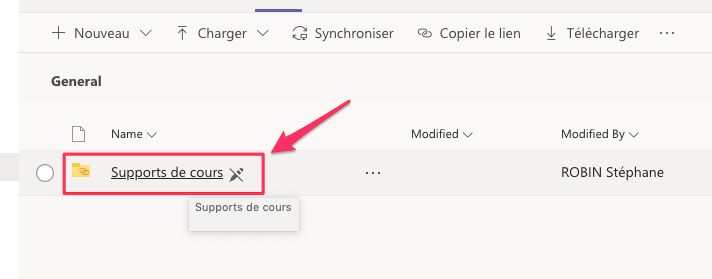
\includegraphics[width=9cm]{./images/teams/ouvrir_dossier_crop}
	\centering
\end{figure}

Vous trouverez dans ce dossier le fichier que votre professeur vous demandera de consulter. Pour le lire, il suffit de cliquer dessus.

\begin{figure}[H]
	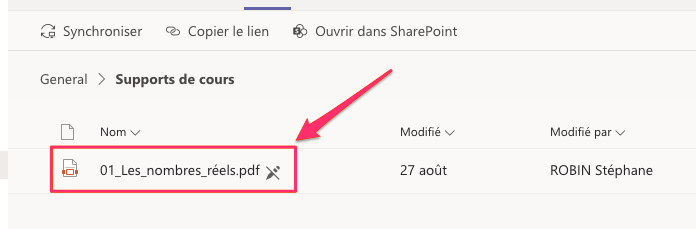
\includegraphics[width=9cm]{./images/teams/ouvrir_fichier_crop}
	\centering
\end{figure}

Vous pouvez à présent consulter le document, mais pas le modifier. Vous pouvez le télécharger pour en garder une copie sur votre ordinateur et éventuellement le modifier par la suite en cliquant sur les trois petits points en haut, puis sur \textit{Télécharger}. Une copie du document apparait alors dans votre dossier Téléchargement.\\

Une fois cela fait, vous pouvez quitter cette page pour revenir à l'affichage du dossier en cliquant sur \textit{Fermer}.
\newpage
\begin{figure}[H]
	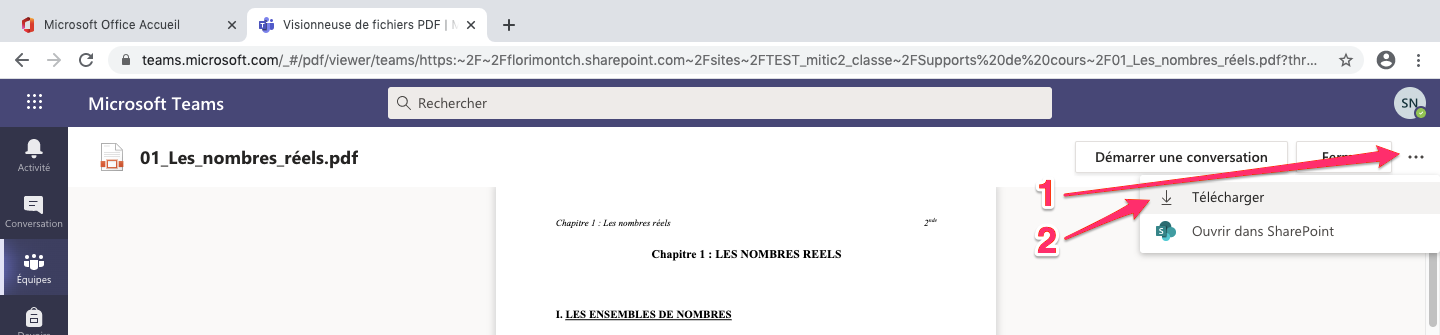
\includegraphics[width=9cm]{./images/teams/telecharger_document_crop}
	\centering
\end{figure}

Il est également possible de télécharger un document depuis la vue du dossier. Il existe plusieurs manières de faire cela. La première consiste à cliquer sur les trois petits points à côté du nom du document, puis sur \textit{Télécharger}.

\begin{figure}[H]
	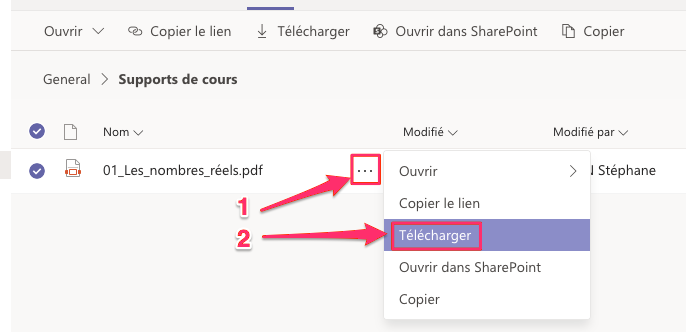
\includegraphics[width=9cm]{./images/teams/telecharger1_crop}
	\centering
\end{figure}

Alternativement, vous pouvez cliquer sur le rond à gauche du nom de fichier pour le sélectionner. Cliquez ensuite sur \textit{Télécharger}, en haut pour télécharger ce fichier. Cette dernière méthode est très pratique si vous désirez télécharger plusieurs fichiers d'un coup, car il suffit alors de les sélectionner puis de cliquer sur \textit{Télécharger} pour les récupérer en même temps.

\begin{figure}[H]
	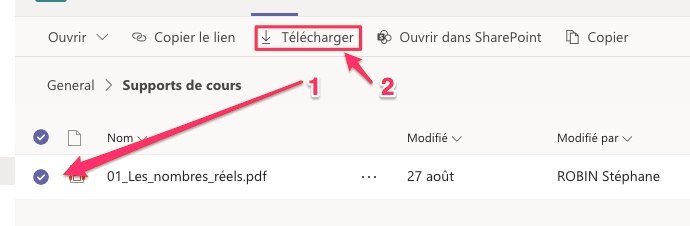
\includegraphics[width=9cm]{./images/teams/telecharger2_crop}
	\centering
\end{figure}



% DEPOSER UN DEVOIR
\section{Les devoirs}

\subsubsection{Consulter le sujet d'un devoir en pièce jointe}\label{consulterDevoir}
Pour consulter les devoirs déposés par votre enseignant, il faut choisir \textit{2 de plus} dans la barre de menus du haut de page, puis sélectionner \textit{Devoirs}.

\begin{figure}[H]
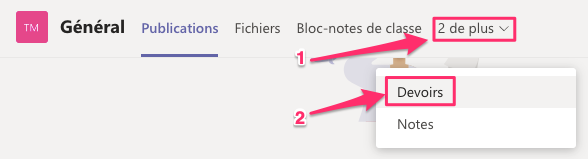
\includegraphics[width=9cm]{./images/teams/devoir1}
\centering
\end{figure}

La page qui s'affiche maintenant fait le bilan de ce qui a déjà été fait et des devoirs proposés par votre enseignant. En cliquant sur \textit{Rédaction} vous pourrez accéder au devoir.

\begin{figure}[H]
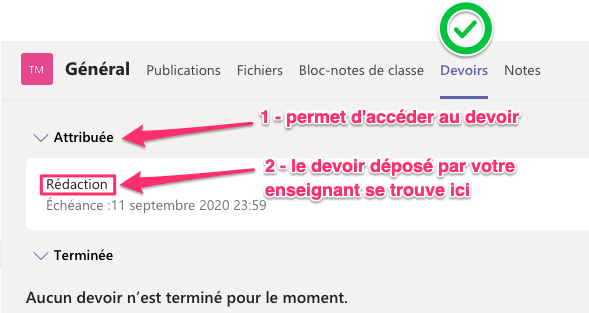
\includegraphics[width=9cm]{./images/teams/devoir2}
\centering
\end{figure}

Vous obtenez alors l'écran suivant

\begin{figure}[H]
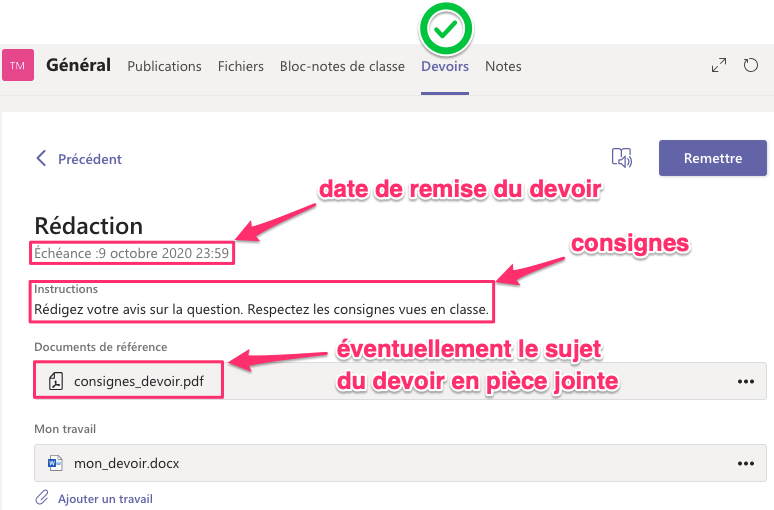
\includegraphics[width=9cm]{./images/teams/devoir3}
\centering
\end{figure}

Il est maintenant possible de consulter le sujet en sélectionnant l'icône 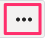
\includegraphics[width=0.7cm]{./images/teams/pointilles} qui vous offre le choix entre une lecture en ligne ou un téléchargement

\begin{figure}[H]
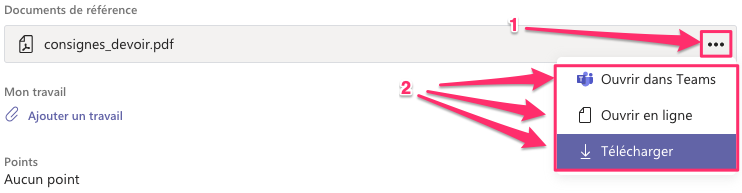
\includegraphics[width=9cm]{./images/teams/choix_pointilles}
\centering
\end{figure}

% REMETTRE SON DEVOIR
\subsection{Remettre son devoir}\label{TeamsRemettreDevoir}

Pour remettre votre devoir, il faut d'abord cliquer sur l'onglet \textit{Ajouter un travail}. 

\begin{figure}[H]
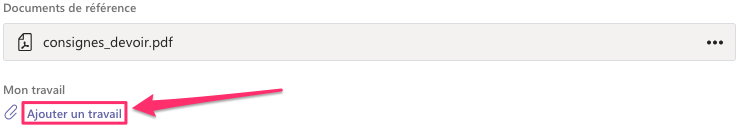
\includegraphics[width=9cm]{./images/teams/ajout}
\centering
\end{figure}

S'ouvre alors une fenêtre qui vous permet de rechercher votre document à partir d'un dossier local relatif à votre ordinateur, à partir du OneDrive ou encore à partir d'une autre équipe.

\begin{figure}[H]
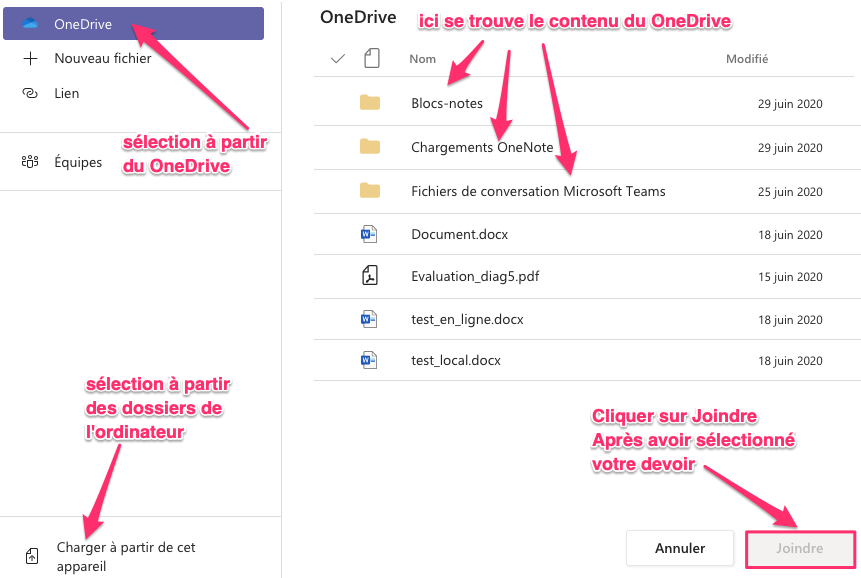
\includegraphics[width=11cm]{./images/teams/selection_devoir}
\centering
\end{figure}

Une fois votre devoir à remettre sélectionné, il suffit de cliquer sur \textit{Joindre}. A ce stade, votre devoir n'est pas encore enregistré. Il faut maintenant choisir \textit{Terminé} pour l'enregistrer.

\begin{figure}[H]
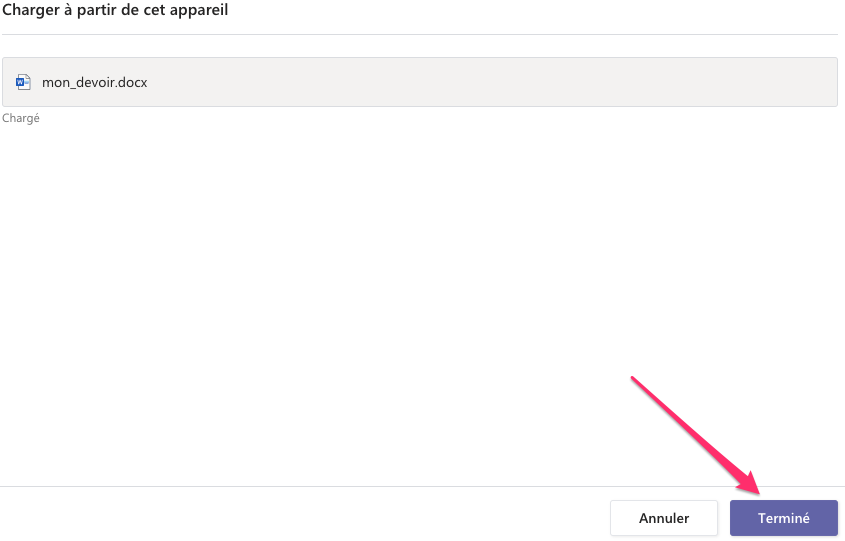
\includegraphics[width=9cm]{./images/teams/ajout2}
\centering
\end{figure}

Vous pouvez également ajouter un autre travail, vous pouvez également télécharger votre devoir afin de vérifier son contenu. Vous pouvez également supprimer votre travail.

\begin{figure}[H]
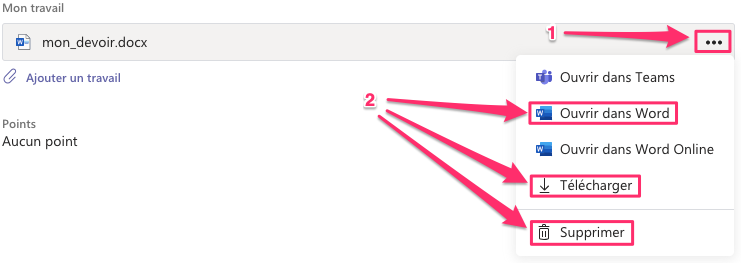
\includegraphics[width=9cm]{./images/teams/ajout3}
\centering
\end{figure}

Attention, votre devoir n'est pas encore remis. il faut maintenant choisir l'onglet \textit{Remettre} pour valider l'envoi de votre devoir. 

\begin{figure}[H]
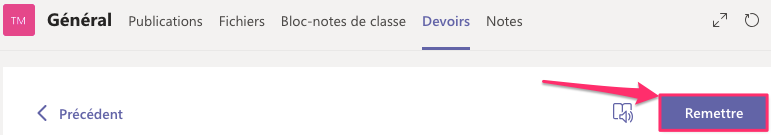
\includegraphics[width=9cm]{./images/teams/ajout4}
\centering
\end{figure}


% ACCEDER A MON CARNET
\section{Accéder à mon bloc-note}

Certains de vos enseignants mettront à votre disposition un bloc-note de classe. C'est un outil très pratique qui permet de prendre des notes et de modifier des fichiers mis à votre disposition, directement depuis Teams.\\

Pour accéder au carnet de classe, cliquez sur \textit{Bloc-notes de classe}, en haut de la page de la classe.

\begin{figure}[H]
	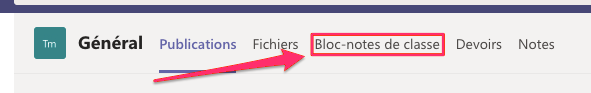
\includegraphics[width=9cm]{./images/teams/acces_bloc_notes_crop}
	\centering
\end{figure}

S'ouvre alors la page d'accueil du bloc-notes. Votre enseignant l'aura probablement adaptée à son cours, elle ne ressemblera donc pas forcément à l'image ci-dessous.

\begin{figure}[H]
	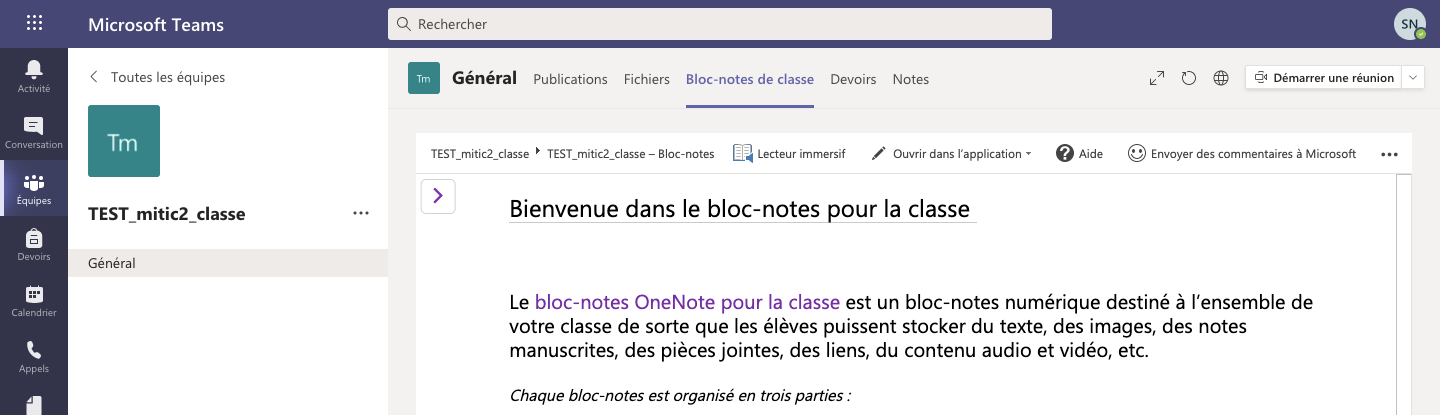
\includegraphics[width=11cm]{./images/teams/ouvrir_menu_bloc_notes_crop}
	\centering
\end{figure}

Cliquez sur la flèche en haut à gauche de l'espace de travail pour ouvrir la liste des bloc-notes. Une section à votre nom apparait, en bas de la liste. Il s'agit d'un espace personnel dans lequel vous pouvez écrire ce que vous voulez, que ce soit pour modifier des fichiers ou prendre des notes. Cliquez sur votre nom pour afficher des sous-sections.

\begin{figure}[H]
	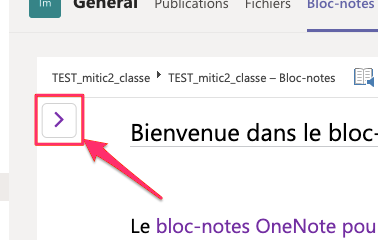
\includegraphics[width=6cm]{./images/teams/ouvrir_liste_dossiers_docs_crop}
	\centering
\end{figure}

Ouvrez la page sans titre, dans la sous-section \textit{Documents}. Ecrivez le titre de votre document. Vous verrez que le titre sera mis à jour dans la liste de documents, à gauche. Si votre liste de sections et documents s'est refermée, il suffit de cliquer sur la flèche, comme tout à l'heure, pour l'afficher à nouveau.\\

Vous pouvez maintenant écrire du texte, ajouter des images, ou modifier ce document comme vous le souhaitez.\\

Si vous souhaitez ajouter une nouvelle page, vous pouvez cliquer sur \textit{+ Page}, en bas. Renommez la nouvelle page en écrivant un titre comme vous venez de le faire.

\begin{figure}[H]
	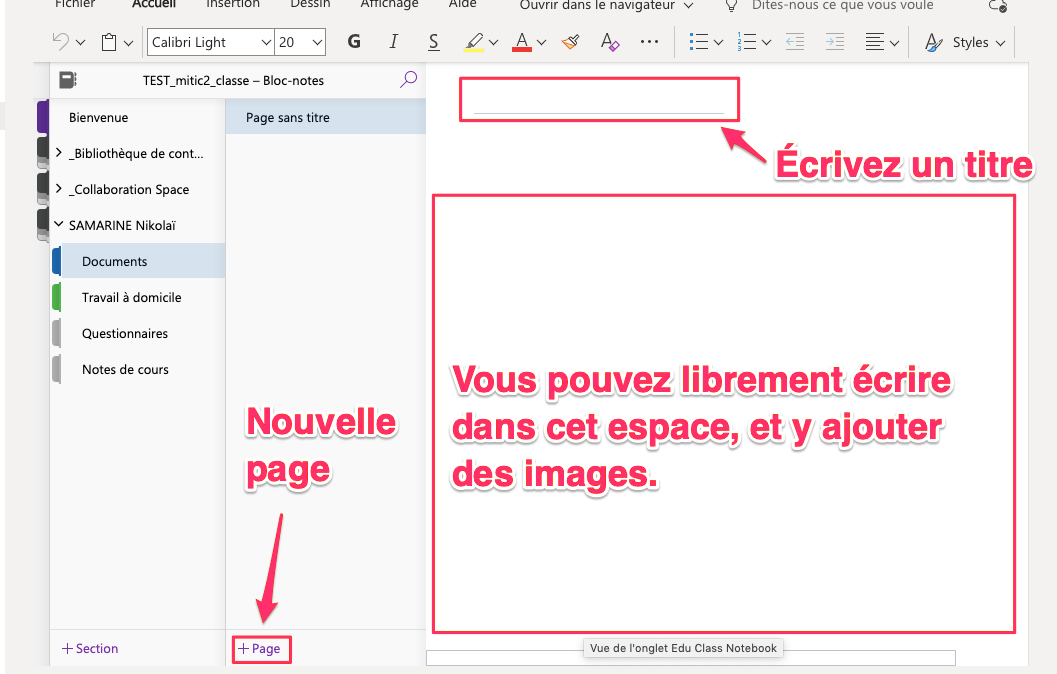
\includegraphics[width=10cm]{./images/teams/sous_section_documents_crop}
	\centering
\end{figure}

En ajoutant et modifiant ainsi des pages, vous allez pouvoir prendre des notes et y accéder via divers appareils, que ce soit depuis la maison ou l'école.

% REJOINDRE UNE VISIO CONFERENCE
\section{Rejoindre une visio-conférence}

Lorsque vous devez assister à un cours à distance, il est nécessaire de rejoindre une visio-conférence déjà commencée. Pour cela, dans l'onglet \textit{Publications}, vous aller trouver une invitation pour participer à une visio-conférence déjà ouverte

\begin{figure}[H]
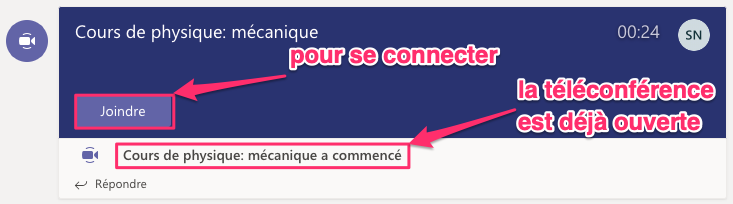
\includegraphics[width=9cm]{./images/teams/video1}
\centering
\end{figure}

Attention, si vous sélectionnez \textit{Demarrer une réunion}, vous allez créer une nouvelle téléconférence et non pas rejoindre la téléconférence déjà programmée pour votre cours.

\begin{figure}[H]
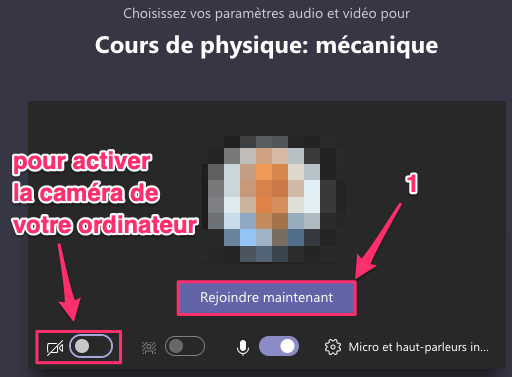
\includegraphics[width=7cm]{./images/teams/video2}
\centering
\end{figure}





% APPARENCE DE LA PAGE D'ACCUEIL
\section{Pour aller plus loin}
\subsection{Apparence de la page d'accueil}

La page d'accueil de Teams se présente sous forme d'une liste d'équipes

\begin{figure}[H]
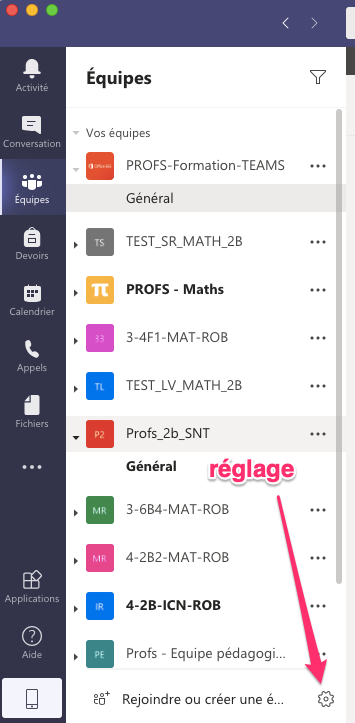
\includegraphics[width=4cm]{./images/teams/accueil_liste}
\centering
\end{figure}

\newpage
ou sous forme d'une grille d'équipes 

\begin{figure}[H]
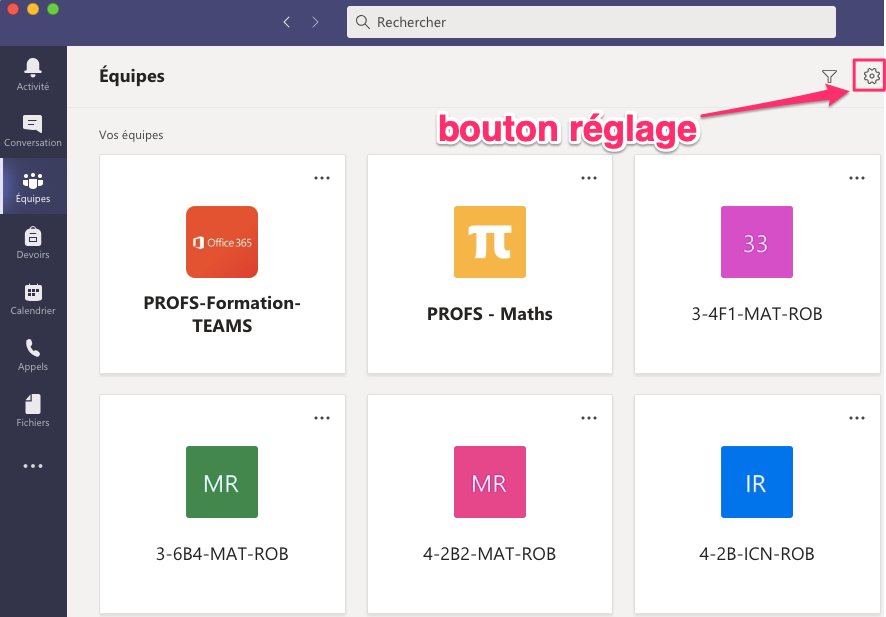
\includegraphics[width=7cm]{./images/teams/accueil_grille}
\centering
\end{figure}

Pour passer d'une forme à l'autre, il faut cliquer sur l'icône 
\includegraphics[width=0.8cm]{./images/teams/bouton_parametres}, choisir \textit{Changer d'affichage} dans le menu déroulant, comme dans l'exemple illustré ci-dessous :

\begin{figure}[H]
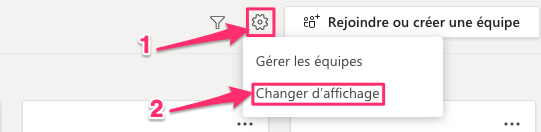
\includegraphics[width=9cm]{./images/teams/changement_liste}
\centering
\end{figure}

Il faut ensuite sélectionner le type d'affichage souhaité entre \textit{Grille} et \textit{Liste}

\begin{figure}[H]
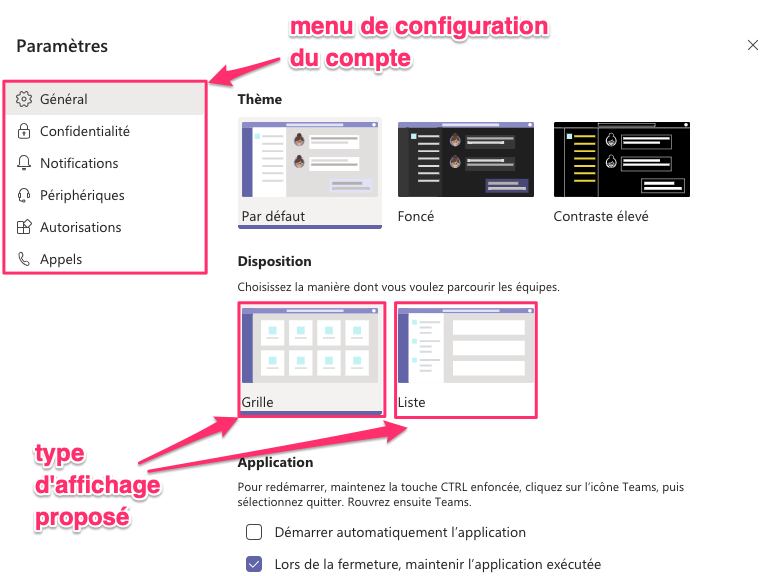
\includegraphics[width=9cm]{./images/teams/choix_parametre}
\centering
\end{figure}

 Pour entrer maintenant dans votre équipe, il suffit de cliquer sur l'icône correspondante

\begin{figure}[H]
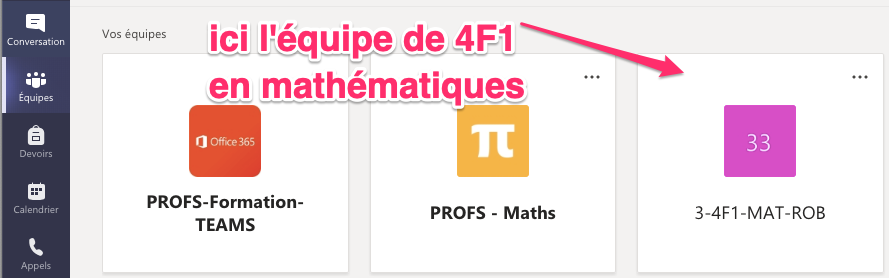
\includegraphics[width=7.5cm]{./images/teams/entree_classe}
\centering
\end{figure}


\chapter{Tableur}  

Un tableur est un logiciel qui permet de faire des calculs à partir de tableaux contenant des nombres (les \emph{données}). Un tableur permet également de représenter ces données sous forme de graphiques qui en facilitent généralement la lecture.

\phantom{rien}

{\footnotesize
\begin{itemize}
\item Logiciel : \emph{Microsoft Excel}
\item Prérequis (se reporter si nécessaire aux \emph{Fiches MITIC 6\up{e}}) :
        \begin{itemize}
        \item insérer une formule ;
        \item utiliser la recopie incrémentale ;
        \item tracer un graphique ;
        \item exporter la feuille et le graphique obtenus.
        \end{itemize}
\item Matières concernées : physique-chimie, mathématiques, histoire-géographie.
\item Compétences : 
        \begin{itemize}
        \item définir le format d'une cellule ;
        \item insérer une courbe de tendance ;
        \item mettre en page une feuille de calcul ;
        \item réaliser un diagramme circulaire ;
        \item exporter un graphique, un tableau.
        \end{itemize}
\item Cette fiche est à réaliser :
        \begin{itemize}
        \item avant les vacances d'octobre en physique-chimie (séance 1) ;
        \item avant les vacances de Noël en mathématiques (séance 2) ;
        \item avant la fin du semestre de cours en géographie (séance 3). 
        \end{itemize}
\end{itemize}
}% fin du footnotesize

\phantom{rien}

Les compétences listées ci-dessous ont été vues en classe de 6\up{e}. Vous en aurez à nouveau besoin pour les activités de cette année. Si nécessaire, reportez-vous aux \emph{Fiches MITIC 6\up{e}} pour revoir comment :  

\begin{itemize}
\item insérer une formule dans une cellule ;
\item utiliser la recopie incrémentale ;
\item tracer un graphique (nuage de points) ;
\item exporter la feuille et le graphique obtenus.
\end{itemize}



%
%
%  S  É  A  N  C  E     I
%
%

\newpage

%\phantom{.} 

%\newpage 

\section{Séance 1 : caractéristique d'une résistance}\label{ficheTableur5e1}


\subsection{Pour bien démarrer...}

Dès que vous avez ouvert un nouveau document dans \emph{Excel}, sauvegardez-le au format Nom-date.xlsx : dans le menu \texttt{Fichier}, choisir \texttt{Enregistrer}. Pendant que vous travaillez, pensez à sauvegarder régulièrement votre travail (raccourci clavier \texttt{Cmd + s}).   

\uneimageici{./images/generales/clavierCmdS}{.4\textwidth}

%\vspace{10pt}

\subsection{L'activité demandée}

\vspace{10pt}

\boiteEnonceLarge{%
Le but de cette séance est de tracer la \emph{caractéristique d'un conducteur ohmique} (une résistance), c'est-à-dire de tracer la droite qui donne l'évolution de la tension $U$ à ses bornes en fonction de l'intensité $I$ du courant qui la traverse. Lors d'un TP de physique, le circuit électrique montré sur le schéma suivant est réalisé.
%
\uneimageici{./images/tableur02/schemaElecR}{.25\textwidth} 
%
L'expérience consiste à faire varier la valeur de la tension $U$ délivrée par le générateur de 0 à 10,0\,V. Pour chacune des valeurs de $U$, on note la valeur du courant $I$ correspondant. Les résultats obtenus sont reportés dans le tableau suivant.  
%
\begin{center}
\begin{tabular}{|c|c|c|c|c|c|c|c|c|c|c|}
\hline
U (V) & 0 & 1,18 & 2,91 & 4,6 & 5,95 & 7,0 & 7,3 & 8,16 & 9,25 & 10,0 \\ \hline
I (mA) & 0 & 17,7 & 42,7 & 68 & 87,6 & 105 & 110 & 124 & 140 & 154 \\ \hline
\end{tabular}
\end{center}
} % fin énoncé



\newpage



\boiteEnonceLarge{
%
Pour réaliser cette activité, vous devrez procéder aux étapes suivantes : 
\begin{enumerate}
\item Créer la feuille de calcul correspondant au tableau de données ci-dessus.
\item Formater les cellules de la première ligne afin que les tensions $U$ soient données avec deux décimales.
\item Formater les cellules de la seconde ligne afin que les intensités $I$ soient données avec une décimale.
\item Tracer le graphique qui représente la tension $U$ en fonction de l'intensité $I$ (c'est-à-dire que l'on souhaite que $U$ soit en ordonnée et que $I$ soit en abscisse).
\item Tracer la droite approchant au mieux tous les points.
\item Par lecture graphique, déterminer quelle est la valeur de l'intensité du courant électrique $I$ lorsque la tension $U=9,00$\,V. Écrire votre réponse dans une cellule de la feuille de calcul, sous le tableau.
\item Par lecture graphique, déterminer la valeur de la tension $U$ lorsque l'intensité du courant électrique vaut $I=100,0$\,mA. Écrire votre réponse dans une cellule de la feuille de calcul, sous la réponse précédente.
\setcounter{tmp}{\value{enumi}}  
\end{enumerate}
%%% ancienne coupure
\begin{enumerate}
\setcounter{enumi}{\value{tmp}}
\item Dans une cellule, ajouter votre prénom, nom et classe.
\item Mettre en forme la feuille de calcul pour que la feuille soit au format \emph{portrait}, avec une marge de 3\,cm en haut, en bas ainsi que sur les côtés. Il faut que tout votre document tienne sur une page uniquement.



%(si nécessaire, se reporter à la fiche méthode \emph{Remettre un devoir sur Moodle}, section \vref{MoodleRendreDevoir}).  
\end{enumerate}
Une fois la mise en forme terminée, vous exporterez votre fichier au format PDF (le fichier doit être nommé à partir de votre nom : \texttt{Nom-date.pdf}), puis vous le rendrez sur \emph{Teams} à l'endroit indiqué par votre enseignant (si nécessaire, se reporter à la fiche méthode \emph{Remettre son devoir}, page \pageref{TeamsRemettreDevoir}).}

\textbf{Pour obtenir de l'aide, rendez-vous à la page \pageref{Tableur5eOutils}}



%\cadre{Pensez à sauver régulièrement votre travail en appuyant sur \texttt{Cmd + s} ou à partir du menu \texttt{Fichier} en choisissant \texttt{Enregistrer}.

%\uneimageici{./images/generales/clavierCmdS}{.4\textwidth}
%}

\vfill
\phantom{rien}




%
%
%  S  É  A  N  C  E     II
%
%


%\pagebreak

\section{Séance 2 : inventaire des tables du collège}\label{ficheTableur5e2}

\subsection{Pour bien démarrer...}

Dès que vous avez ouvert un nouveau document dans \emph{Excel}, sauvegardez-le au format Nom-date.xlsx : dans le menu \texttt{Fichier}, choisir \texttt{Enregistrer}. Pendant que vous travaillez, pensez à sauvegarder régulièrement votre travail (raccourci clavier \texttt{Cmd + s}).   

\uneimageici{./images/generales/clavierCmdS}{.4\textwidth}

%\vspace{10pt}

\subsection{L'activité demandée}

\vspace{10pt}

\boiteEnonceLarge{%
Le but de cette séance est de tracer un diagramme circulaire pour représenter un état des lieux des tables d'un collège.\\ %Pour parvenir à ce résultat, vous devrez utiliser les outils présentés en début de chapitre (voir section \vref{Tableur5eOutils}).\\[4pt]
%

Le gestionnaire d'un établissement fait l'état des lieux et vérifie l'état des tables :

\begin{center}
\begin{tabular}{lcl}
$\bullet$ 132 sont neuves ;& & $\bullet$ 55 sont à réparer ; \\
$\bullet$ 231 sont en bon état ;&  & $\bullet$ 33 sont à changer.\\
$\bullet$ 99 sont dans un état passable ;& & \\
\end{tabular}
\end{center}
%
} % fin énoncé

\vfill
\phantom{rien}
%\newpage



\boiteEnonceLarge{%
Pour réaliser cette activité, vous devrez procéder aux étapes suivantes :
\begin{enumerate}
\item Créer la feuille de calcul suivante :
\uneimageici{./images/tableur02/ActiviteMaths1}{.75\textwidth}
\vspace{-8pt}
\item Compléter la deuxième ligne du tableau ci-dessous avec les données de l'énoncé.
\item Quelle formule faut-il utiliser pour calculer automatiquement la valeur attendue dans la cellule \texttt{G2} ?
\item Quelle formule faut-il utiliser dans la cellule \texttt{B3} pour calculer la fréquence des tables neuves ?
        \begin{enumerate}
        \item Programmer alors toutes les cellules de la ligne en effectuant une recopie incrémentale.
        \item Que se passe-t-il alors ?
        \end{enumerate}
        \emph{En cliquant sur la cellule \texttt{C3}, on remarque que le nombre de chaises est divisé par le contenu de la cellule \texttt{H2}. Pour éviter ce problème, il faut dans la cellule \texttt{B3} avant la recopie incrémentale insérer un signe \texttt{\$} devant la lettre \texttt{G} comme suit : \texttt{\$G2}. Ceci a pour effet d'empêcher l'incrémentation de l'index de cellule précédé du \texttt{\$}.} 
\item Comment obtenir la fréquence en pourcentage à partir de la fréquence ? Programmer alors les cellules de la ligne 4 à l'aide d'une instruction.
\item Insérer dans le fichier un diagramme circulaire permettant au gestionnaire de présenter cet état des lieux.
\setcounter{tmp}{\value{enumi}}  
\end{enumerate}
% ancienne coupure
\begin{enumerate}
\setcounter{enumi}{\value{tmp}}
\item Le gestionnaire veut réaliser ce diagramme circulaire à la main sur du papier. Pour cela, il faut ajouter dans le fichier la ligne suivante :
%
\uneimageici{./images/tableur02/ActiviteMaths2}{.75\textwidth}
%
\vspace{-8pt} Quel nombre faut-il saisir dans la cellule \texttt{G5} ?
%

\item En utilisant uniquement les valeurs de la ligne 3 et de la cellule \texttt{G5}, programmer les cellules \texttt{B5} à \texttt{F5} pour obtenir les angles voulus. Modifier le format de cellule pour arrondir les angles à l'unité.
\item En changeant uniquement la valeur d'une cellule, il est possible d'obtenir les angles permettant de construire un diagramme semi-circulaire. Quelle est cette cellule ? Quelle valeur faut-il mettre ?
\item Mettre en forme la feuille de calcul pour que la feuille soit au format \emph{portrait}, avec une marge de 3\,cm en haut et en bas, et de 2\,cm sur les côtés. Il faut que tout le document tienne sur une page uniquement.
\item Supprimer l'en-tête et le pied de page par défaut. 
\item\label{questionDiagDemiCirc} Construire ensuite (et à la main !) le diagramme semi-circulaire correspondant ci-dessous.
\end{enumerate}}

\boiteEnonceLarge{
Une fois la mise en forme terminée, vous exporterez votre fichier au format PDF (le fichier doit être nommé à partir de votre nom : \texttt{Nom-date.pdf}), puis vous le rendrez sur \emph{Teams} à l'endroit indiqué par votre enseignant (si nécessaire, se reporter à la fiche méthode \emph{Remettre son devoir}, page \pageref{TeamsRemettreDevoir}).}

Construire ici le diagramme semi-circulaire de la question \ref{questionDiagDemiCirc}   :

\uneimageici{./images/tableur02/hemicercle}{.4\textwidth}   

\textbf{Pour obtenir de l'aide, rendez-vous à la page \pageref{Tableur5eOutils}}

%\vfill

%\cadre{Pensez à sauver régulièrement votre travail en appuyant sur \texttt{Cmd + s} ou à partir du menu \texttt{Fichier} en choisissant \texttt{Enregistrer}.}

\vfill


\phantom{rien} 




%
%
%  S  É  A  N  C  E     III
%
%

\newpage

%\pagebreak

\section{Séance 3 : répartition de la population mondiale}\label{ficheTableur5e3}

\subsection{Pour bien démarrer...}

Dès que vous avez ouvert un nouveau document dans \emph{Excel}, sauvegardez-le au format Nom-date.xlsx : dans le menu \texttt{Fichier}, choisir \texttt{Enregistrer}. Pendant que vous travaillez, pensez à sauvegarder régulièrement votre travail (raccourci clavier \texttt{Cmd + s}).   

\uneimageici{./images/generales/clavierCmdS}{.4\textwidth}


\subsection{L'activité demandée}


\vspace{10pt}
\boiteEnonceLarge{%
Le but de cette séance est de tracer un diagramme circulaire pour représenter la répartition de la population mondiale par continent. %Pour parvenir à ce résultat, vous devrez utiliser les outils présentés en début de chapitre (voir section \vref{Tableur5eOutils}).\\[12pt]
%

La carte ci-dessous\footnote{D'après \url{http://icdc.us}, consulté le 5 juillet 2017 et remis à jour avec les données de la page Wikipédia \emph{Population mondiale}, consultée le 5 juillet 2017.} donne la répartition par zone géographique de la population mondiale en 2017 (en nombre d'habitants).

\uneimageici{./images/tableur02/cartePopulation}{.9\textwidth}
}

\boiteEnonceLarge{
À partir de ce document, vous devez créer un diagramme circulaire montrant cette répartition. Pour cela, il faut suivre les étapes suivantes.

\begin{enumerate}
\item Créer une feuille de calcul contenant les données fournies par le document ci-dessus. Attention, il faut sommer les populations d'Amérique du Nord et d'Amérique du Sud car on souhaite avoir la répartition par continent.
\item Dans une nouvelle colonne, transformer les populations en pourcentage à l'aide d'une formule. Il suffit d'écrire la formule pour la première cellule de la colonne et ensuite utiliser une recopie incrémentale (se reporter si nécessaire aux fiches Mitic 6\up{e}) pour que la formule s'applique à toutes les cellules de la colonne.
%\setcounter{tmp}{\value{enumi}}  

%\setcounter{enumi}{\value{tmp}}
\item Ajouter un formatage de cellule : choisir \texttt{Nombre} pour la colonne contenant les données en \%\ et régler le nombre de décimale à 0.
\item À partir des données en \%\ calculées, construire un diagramme circulaire montrant la répartition de la population mondiale par continent.
\item Mettre en forme la feuille de calcul pour que la feuille soit au format \emph{portrait}, avec une marge de 3\,cm en haut et en bas, et de 2\,cm sur les côtés. Il faut que tout votre document tienne sur une page uniquement.
\end{enumerate}
Une fois la mise en forme terminée, vous exporterez votre fichier au format PDF (le fichier doit être nommé à partir de votre nom : \texttt{Nom-date.pdf}), puis vous le rendrez sur \emph{Teams} à l'endroit indiqué par votre enseignant (si nécessaire, se reporter à la fiche méthode \emph{Remettre son devoir}, page \pageref{TeamsRemettreDevoir}).}

\textbf{Pour obtenir de l'aide, rendez-vous à la page \pageref{Tableur5eOutils}}
%\vfill

%\cadre{Pensez à sauver régulièrement votre travail en appuyant sur \texttt{Cmd + S} ou à partir du menu \texttt{Fichier} en choisissant \texttt{Enregistrer}.

%\uneimageici{./images/generales/clavierCmdS}{.5\textwidth}
%}

\vfill
\phantom{rien}


\newpage
% AIDE

\section{Aide pour réaliser les activités}\label{Tableur5eOutils}
 
Les nouveaux outils dont vous aurez besoin pour réaliser les trois séances sur le tableur sont décrits ci-dessous :

\begin{itemize}  
\item séparateur décimal, voir section \vref{Calc2SeparateurDecimal}  
\item formater le contenu d'une cellule, voir section \vref{Calc2FormaterCellule} ;
\item formater la page, voir section \vref{Calc2FormaterPage} ;
\item ajouter une courbe de tendance sur un graphique, voir section \vref{Calc2CourbeTendance} ;
\item créer un diagramme circulaire, voir section \vref{Calc2DiagCirculaire}.
\end{itemize}  

\subsection{Le séparateur décimal}\index{Calc!Séparateur décimal}\index{Séparateur décimal (Calc)}\index{Calc!Changer les points en virgules}\index{Changer les points en virgules (Calc)}\index{Virgule ou point ? (Calc)}\label{Calc2SeparateurDecimal}


%%%%%%%%%%%%%%%%%%%%%

\subsubsection{Quel est votre séparateur décimal ?}


Le \emph{séparateur décimal} est le caractère utilisé pour écrire les nombres à virgule. En fonction de la langue du système d'exploitation de l'ordinateur on utilise pour les systèmes anglo-saxons, le point (ex. : $4.5$) ou pour les systèmes francophones, la virgule (ex. : $4,5$).

\vspace{6pt}

Dans Excel, on peut déterminer si on utilise un point ou une virgule comme séparateur décimal. Pour cela, faire le test suivant : dans différentes cellules écrire un texte, un nombre entier et un nombre à virgule en utilisant une virgule puis un point. Les textes sont alignés à gauche et les nombres à droite. Dans les exemples ci-dessous, le séparateur décimal est donc la virgule pour l'image de gauche (le logiciel installé sur l'ordinateur) et le point pour l'image de droite (le logiciel accédé via office.com). Dans le premier cas, $3,14$ est reconnu comme un nombre et se retrouve aligné à droite, alors que $3.14$ se voit transformé en date (le 14 mars).

\uneimageici{./images/tableur02/SeparateurDecimal_excel}{.2\textwidth}

Avant de faire une activité sur Excel, pensez à vérifier si le séparateur décimal est le point ou la virgule chez vous. Tous les exemples de cet ouvrage utilisent le séparateur décimal francophone, la virgule. Si vous désirez avec le séparateur anglophone, le point, n'oubliez pas de remplacer les virgules par des points lorsque vous les copiez.

\subsubsection{Changer les virgules en points (ou inversement)}

Parfois il est nécessaire de changer toutes les virgules en points (ou inversement). Pour cela, dans le menu \texttt{Édition}, choisir \texttt{Rechercher} puis \texttt{Remplacer...}

\uneimageici{./images/tableur02/changerVirgule1_excel_crop}{.35\textwidth}

Dans la boîte de dialogue qui s'ouvre (figure ci-dessous), indiquer le caractère à rechercher \circled{1} (ici la virgule) et le caractère de remplacement \circled{2} (ici le point). Pour terminer, cliquer sur \texttt{Remplacer tout} \circled{3} ce qui aura pour effet de remplacer en une fois tous les points du document.

\emph{Remarque : en cliquant sur \texttt{Remplacer}, une confirmation est demandée avant le remplacement de chaque point.}

\uneimageici{./images/tableur02/changerVirgule2_excel_crop}{.8\textwidth}

%%%%%%%%%%%%%%%%%%%%%%%%%%

\subsection{Formater le contenu d'une cellule}\index{Calc!Formater le contenu d'une cellule}\index{Formater le contenu d'une cellule (Calc)}\label{Calc2FormaterCellule} 

\emph{Formater} le contenu d'une cellule signifie choisir le \emph{format} des données qu'elle contient. Par exemple, si une cellule contient le résultat du calcul $\frac{1}{3}$, on n'a pas forcément envie que le nombre affiché soit $0,3333333333$, mais plutôt un nombre arrondi au centième, comme par exemple $0,33$. On peut alors \emph{formater} la cellule et demander que le nombre ne soit affiché qu'avec deux décimales.

Pour formater des cellules, il faut tout d'abord les sélectionner (on peut sélectionner une seule cellule, plusieurs cellules ou encore toute une ligne ou une colonne).

\cadre{Dans un tableur, pour sélectionner :
\begin{itemize}
\item une ligne entière, il faut cliquer sur le numéro de la ligne à gauche de la fenêtre ;
\item une colonne entière, il faut cliquer sur la lettre au sommet de la colonne ;
\item toute la feuille de calcul, il faut cliquer dans la case au-dessus du \texttt{1} et à gauche du \texttt{A} dans la feuille de calcul.  
\end{itemize}} 

\uneimageici{./images/tableur02/FormatCellule1_Excel_crop}{.3\textwidth}

Pour accéder à la boîte de dialogue permettant de formater les cellules, deux solutions :
\begin{itemize}
\item dans le menu \texttt{Mise en forme}, choisir \texttt{Cellule...} (figure ci-dessous à gauche) ;    
\item effectuer un clic droit sur les cellules sélectionnées et choisir \texttt{Format de cellule...} (figure ci-dessous à droite).
\end{itemize}

\deuximagesici{./images/tableur02/FormatCellule3_Excel_crop}{1.15\textwidth}%  
              {./images/tableur02/FormatCellule2_Excel_crop}{.65\textwidth}

Dans la boîte de dialogue qui s'ouvre (figure ci-dessous), choisir l'onglet \texttt{Nombres} (sur l'image ci-dessous, \circled{1}), puis la catégorie \texttt{Nombre} \circled{2}. On peut alors régler le \texttt{Nombre de décimales} \circled{3} et un \texttt{Séparateur de milliers}\footnote{Le séparateur de milliers ajoute un espace qui permet une lecture plus facile des nombres. Ainsi, 19402445 sera écrit 19 402 445.} \circled{4}. Une fenêtre permet d'observer le résultat du réglage \circled{5}. Terminer en cliquant sur le bouton \texttt{OK} \circled{6}.              

\uneimageici{./images/tableur02/FormatCellule4_Excel_crop2}{.8\textwidth}  



\subsection{Formater la page}\index{Calc!Formater la page}\index{Formater la page (Calc)}\label{Calc2FormaterPage} 

\emph{Formater la page} permet de choisir les marges, mais aussi l'en-tête et le pied de page, qui seront utilisées autour de la page. Cela est en particulier important pour une impression papier ou un export au format PDF, mais permet également de définir le nombre de pages qui doivent être utilisées (voulez-vous toute la feuille de calcul sur une seule page, ou sur deux pages en largeur ?).

\vspace{12pt}

Pour formater la page, ouvrir la barre de \texttt{Mise en page}, en haut de la fenêtre. 

\uneimageici{./images/tableur02/FormatPage1_Excel_crop}{.8\textwidth}



\subsubsection{Orientation et marges}  

Dans la boîte de dialogue qui s'ouvre, se rendre dans l'onglet \texttt{Page} pour choisir les marges \circled{1} et l'orientation de la page \circled{2}.

\deuximagesPGici{./images/generales/portraitPaysage}{\textwidth}%
                {./images/tableur02/FormatPage4_Excel_crop}{\textwidth}  


\subsubsection{Nombre de pages}

Pour choisir le nombre de pages sur lequel le document va apparaître, il faut utiliser les options \texttt{Largeur} et \texttt{Hauteur}, à droite du ruban \texttt{Mise en page}. Par défaut, ce sont les tailles automatiques qui génèrent assez de pages pour afficher toutes les cellules avec du contenu de la feuille. Choisir un nombre permet soit de forcer l'impression d'un nombre supérieur de page soit d'ignorer certaines cellules situées au-delà des premières pages. Par exemple, choisir \texttt{1 page} dans les deux options permet de n'imprimer qu'une page.

\uneimageici{./images/tableur02/FormatPage5_Excel_crop}{.8\textwidth} 



\subsubsection{En-tête et pied de page}

Pour modifier l'en-tête du document, il faut choisir \texttt{Mise en page}, toujours dans le ruban \texttt{Mise en page}.
\uneimageici{./images/tableur02/FormatPage5a_Excel_crop}{.8\textwidth} 

D'abord, cliquer sur l'onglet \texttt{En-tête/Pied de page} \circled{1}. Là, on peut choisir un type d'en-tête \circled{2}, dont un visuel s'affiche en dessous \circled{3}. Pour personnaliser l'en-tête, il faut sélectionner \texttt{En-tête personnalisé...} \circled{4}.

\uneimageici{./images/tableur02/FormatPage5b_Excel_crop}{.8\textwidth}  

Quand on clique sur \texttt{En-tête personnalisé...}, on obtient la fenêtre ci-dessous. On peut directement taper le texte qui apparaîtra en haut à gauche de la page en l'écrivant dans la section \texttt{Section de gauche} \circled{1}. On peut, de même, déterminer le texte qui apparaît au centre ou à droite en écrivant dans les sections correspondantes. Une série d'icônes en haut de la fenêtre permet notamment : de mettre en forme le texte \circled{2}, d'insérer le numéro de la page \circled{3} ou d'insérer le nombre total de pages du document \circled{4}.


\uneimageici{./images/tableur02/FormatPage6_Excel_crop}{.8\textwidth}  

Dans la fenêtre \texttt{Pied de page personnalisé...}, on retrouve les mêmes options pour modifier l'aspect du pied de page.





\subsection{Ajouter une courbe de tendance}\index{Calc!Ajouter courbe de tendance}\index{Ajouter une courbe de tendance (Calc)}\label{Calc2CourbeTendance} 

Dans le cas d'un graphique, comme représenté sur la figure ci-dessous, la \emph{courbe de tendance linéaire} est la droite qui s'approche au mieux de tous les points. 

\uneimageici{./images/tableur02/graphiqueObtenu1_Excel_crop}{.6\textwidth} 


Pour ajouter une courbe de tendance, sélectionner les points du graphique en cliquant dessus, puis effectuer un clic droit et choisir dans le menu contextuel \texttt{Ajouter une courbe de tendance...}

\uneimageici{./images/tableur02/ajoutCourbeTendance1_Excel_crop}{.5\textwidth}%

Un espace de personnalisation s'ouvre sur la droite de votre fenêtre. Choisissez l'option de courbe \texttt{Linéaire} \circled{1}. Vous pouvez apercevoir votre courbe de tendance apparaître sur votre graphique \circled{2}. Si vous voulez personnaliser votre courbe de tendance, vous pouvez cliquer sur les deux onglets en haut de cet espace \circled{3}.

\uneimageici{./images/tableur02/ajoutCourbeTendance2_Excel_crop}{.4\textwidth} 


\subsection{Créer un diagramme circulaire}\index{Calc!Créer un diagramme circulaire}\index{Créer un diagramme circulaire (Calc)}\label{Calc2DiagCirculaire}

Un \emph{diagramme circulaire} est une représentation graphique qui permet une visualisation rapide et très efficace des données. En effet, lire que l'air est composé de 78\,\% de diazote, de 21\,\% de dioxygène, de 0,9\,\% d'argon et enfin de 0,1\,\% d'autres gaz, est beaucoup moins marquant que regarder le diagramme circulaire ci-dessous montrant la composition de l'air.

\uneimageici{./images/tableur02/InsererDiagramme4_Excel_crop}{.4\textwidth}

Pour créer un diagramme circulaire, il faut tout d'abord sélectionner les données à représenter \circled{1}, puis dans le menu \texttt{Insertion} \circled{2}, cliquer sur l'icône représentant un graphique circulaire \circled{3}. S'ouvre alors une liste de différents types de diagrames circulaires. Cliquer sur le premier des \texttt{Secteurs 2D}. Votre graphique apparait alors dans la feuille de calcul.

\uneimageici{./images/tableur02/InsererDiagramme1_Excel_crop}{.6\textwidth}



\chapter{Traitement de texte}  

Un traitement de texte est un logiciel qui permet d'effectuer la mise en forme d'un texte : choix d'une police de caractères, de sa taille, de sa couleur, mise en forme de la page, des marges, des pieds de page, des entêtes, mise en forme des paragraphes, création de listes à puces, de listes numérotées, ou encore toute fonctionnalité permettant de personnaliser le contenu d'un document.\\

{\footnotesize
\begin{itemize}
\item Logiciel\footnote{Le logiciel Microsoft Word est téléchargeable : \url{http://www.microsoft.com/}} : \emph{Microsoft Word} 
\item Prérequis (se reporter si nécessaire aux \emph{Fiches MITIC 6\up{e}}) : 
        \begin{itemize}
        \item mettre en forme des caractères, des paragraphes et des pages ;
        \item insérer une image dans un texte ;
        \item exporter au format PDF.
        \end{itemize}
\item Matières concernées : français, anglais, histoire.
\item Compétences : 
        \begin{itemize}
        \item insérer un tableau et définir ses propriétés ;
        \item insérer une liste à puces ;
        \item insérer un lien hypertexte vers un site internet ;
        \item utiliser le correcteur d'orthographe ;
        \item insérer une image et adapter le texte autour de l'image.
        \end{itemize}
\item Cette fiche est à réaliser :
        \begin{itemize}
        \item avant les vacances d'octobre en français (séance 1) ;
        \item avant les vacances de printemps en anglais (séance 2) ;
        \item avant la fin du semestre de cours en histoire (séance 3). 
        \end{itemize}
\end{itemize}
}% fin du footnotesize

\phantom{rien}

% \hfill 
\includegraphics[width=3cm]{./images/generales/VuEn6e}

Les compétences listées ci-dessous ont été vues en classe de 6\up{e}. Vous en aurez à nouveau besoin pour les activités de cette année. Si nécessaire, reportez-vous aux \emph{Fiches MITIC 6\up{e}} pour revoir comment :  

\begin{itemize}
\item mettre en forme la page ;
\item mettre en forme des caractères (police, italique, gras, souligné, couleur du texte) ;
\item mettre en forme des paragraphes (aligner à gauche ou à droite, justifier, retraits et espacements autour du paragraphe, encadrement) ;
\item insérer une image dans un texte (retailler l'image, conserver le ratio) ;
\item exporter un document au format PDF.
\end{itemize}







%
%
%  S  É  A  N  C  E     I
%
%

\newpage

\section{Séance 1 : mise en forme d'un texte en français}\label{ficheTexte5e1}

\subsection{Pour bien démarrer...}

Dès que vous avez ouvert un nouveau document dans \emph{Word}, sauvegardez-le au format Nom-date.docx : dans le menu \texttt{Fichier}, choisir \texttt{Enregistrer}. Pendant que vous travaillez, pensez à sauvegarder régulièrement votre travail (raccourci clavier \texttt{Cmd + s}).   

\uneimageici{./images/generales/clavierCmdS}{.4\textwidth}

\subsection{L'activité demandée}

\vspace{10pt}

\boiteEnonceLarge{Le but de cette séance est de mettre en forme un extrait de \emph{La chanson de Roland}, dont une version <<\,brute\,>> est disponible sur la page Teams de votre cours. Le modèle à obtenir est montré ci-dessous. Pour parvenir à ce résultat, vous devrez effectuer les étapes suivantes :
%
\begin{enumerate}
\item Récupérer la version brute du document sur la page Teams de votre cours.
\item Ajouter le tableau au début du document, et le compléter.
\item Mettre en forme la page (marges de 2\,cm en haut et 3\,cm en bas, à gauche et à droite).
\item Mettre en forme le texte comme montré ci-dessous. Entre autres, le nom des personnages apparaît dans la liste à puces en gras et dans le texte, en italique. 
\item Ajouter un lien hypertexte pour le titre \og La chanson de Roland \fg qui pointe vers la page Wikipédia de cette œuvre : \url{https://fr.wikipedia.org/wiki/Chanson_de_Roland}.
\item Ajouter les trois notes de bas de page.
\item Sur la page Wikipédia de l'œuvre, récupérer l'image : pour cela effectuer un clic droit sur l'image, puis choisir \texttt{Enregistrer l'image sous...} dans le menu contextuel qui s'ouvre. Enregistrer l'image sur le \texttt{Bureau} de l'ordinateur afin de la retrouver facilement, puis l'insérer et la positionner dans le texte.
\end{enumerate}
Une fois la mise en forme terminée, vous exporterez votre fichier au format PDF (le fichier doit être nommé à partir de votre nom : \texttt{Nom-date.pdf}), puis vous le rendrez sur \emph{Teams} à l'endroit indiqué par votre enseignant (si nécessaire, se reporter à la fiche méthode \emph{Remettre son devoir}, page \pageref{TeamsRemettreDevoir}).}



%\vfill
\vfill
\phantom{rien}

\begin{center}\fbox{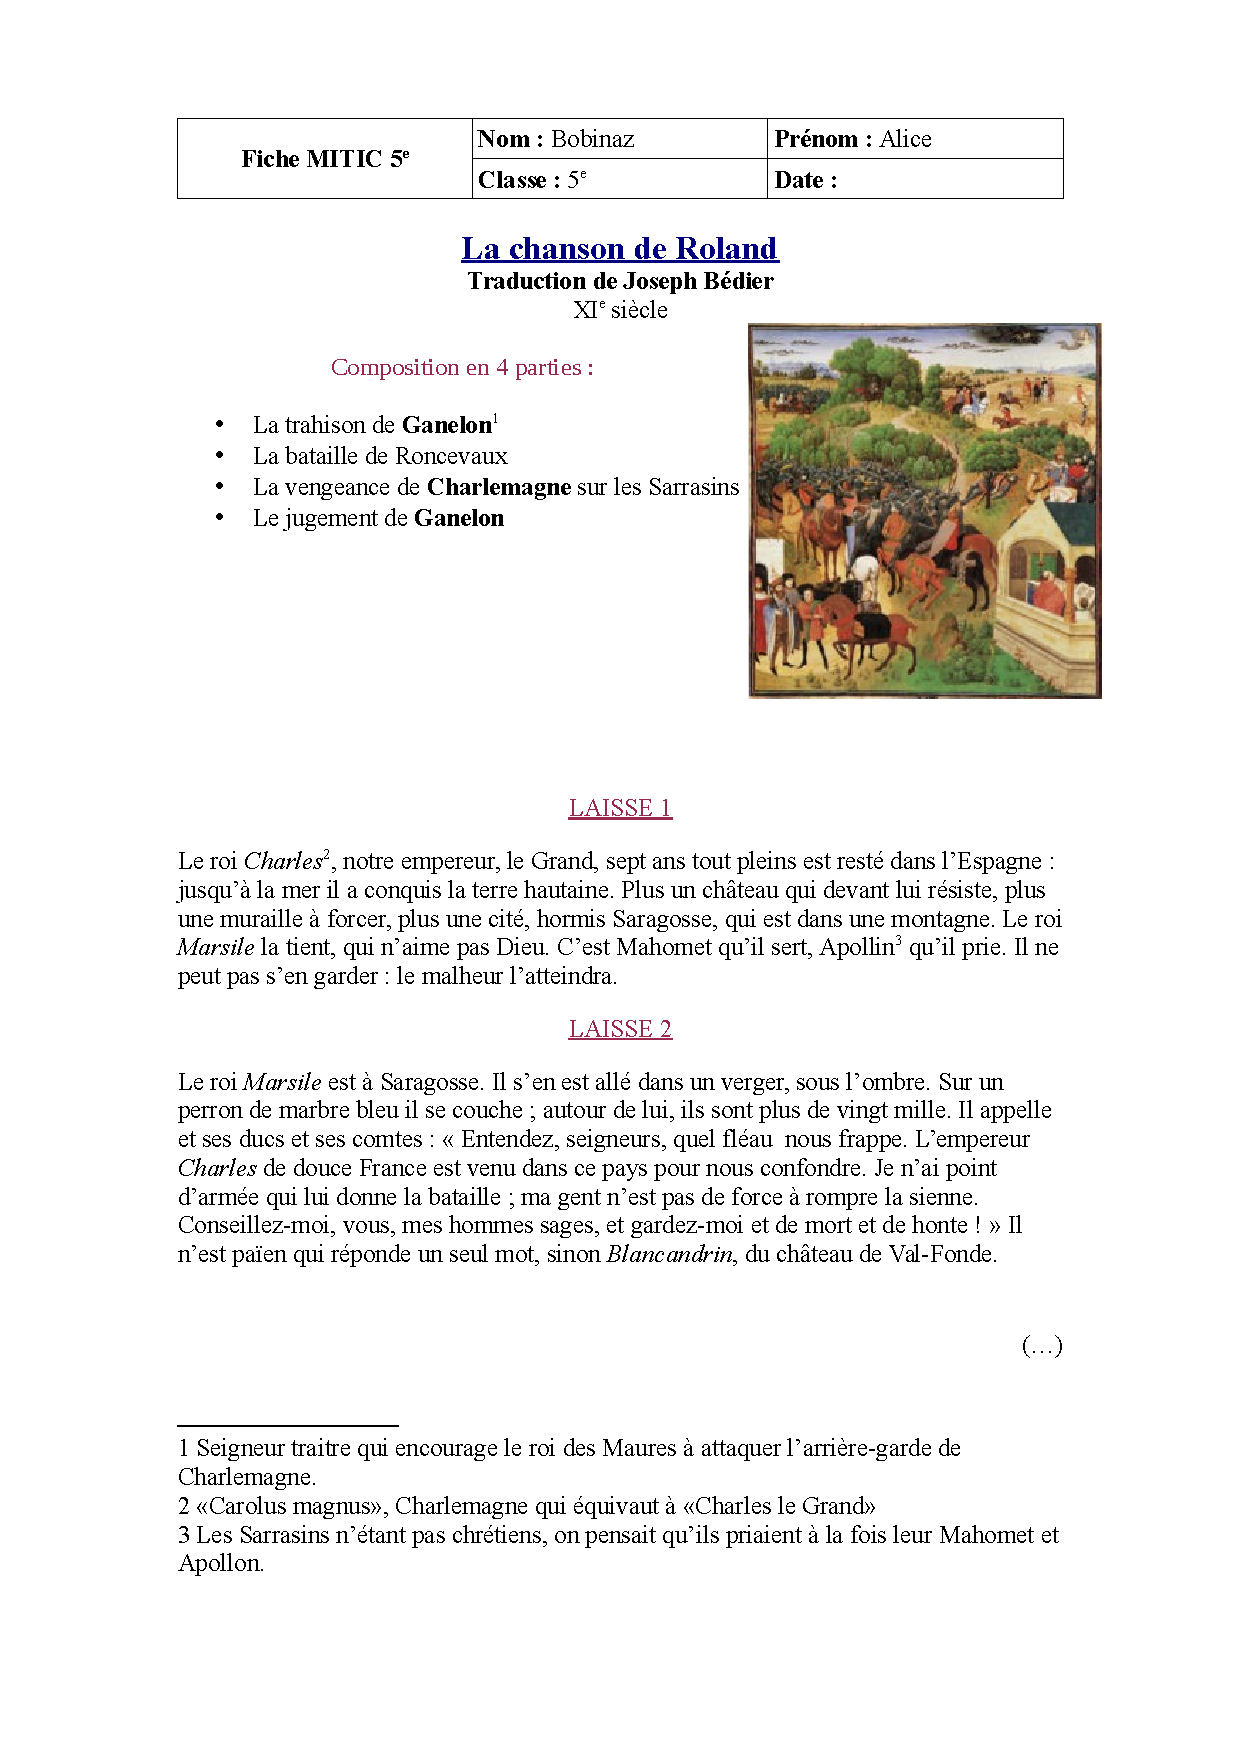
\includegraphics[width=.75\textwidth]{./sources/texte02/ExtraitChansonRoland5eFormate}}\label{modelePage5e1}\end{center}

\textbf{Pour obtenir de l'aide, rendez-vous à la page \pageref{aide_seancesWord}}

%\cadre{Pensez à sauver régulièrement votre travail en appuyant sur \texttt{Cmd + s} ou à partir du menu \texttt{Fichier} en choisissant \texttt{Enregistrer}.

%\uneimageici{./images/generales/clavierCmdS}{.3\textwidth}
%}

%\newpage


%\phantom{rien} 


%\vfill



%\vfill

%\phantom{rien} 




%
%
%  S  É  A  N  C  E     II
%
%


\newpage

\section{Séance 2 : mise en forme d'un texte en anglais}\label{ficheTexte5e2}

\subsection{Pour bien démarrer...}

Dès que vous avez ouvert un nouveau document dans \emph{Word}, sauvegardez-le au format Nom-date.docx : dans le menu \texttt{Fichier}, choisir \texttt{Enregistrer}. Pendant que vous travaillez, pensez à sauvegarder régulièrement votre travail (raccourci clavier \texttt{Cmd + s}).   

\uneimageici{./images/generales/clavierCmdS}{.4\textwidth}

\subsection{L'activité demandée}

%\vspace{10pt}

\boiteEnonceLarge{Le but de cette séance est de mettre en forme un extrait d'une œuvre de Shakespeare, \emph{Much Ado About Nothing}, dont une version <<\,brute\,>> est disponible sur la page Teams de votre cours. Le modèle à obtenir est montré ci-dessous. Pour parvenir à ce résultat, vous devrez effectuer les étapes suivantes :
\begin{enumerate}
\item Récupérer la version brute du document sur la page Teams de votre cours.
\item Ajouter le tableau au début du document, et le compléter.
\item Mettre en forme la page avec des marges de 2\,cm en haut, en bas, à gauche et à droite.
\item Mettre en forme le texte comme montré page ci-contre. Entre autres, les personnages sont présentés dans une liste à puces et dans le texte, leur nom apparaît en italique.
\item Ajouter un lien hypertexte pour le titre "Much Ado About Nothing" qui pointe vers la page Wikipédia de cette œuvre : \url{https://en.wikipedia.org/wiki/Much_Ado_About_Nothing}.
\item Ajouter les notes de bas de page qui donnent la traduction de mots difficiles (vous pouvez en ajouter d'autres).
\item Sur la page Wikipédia anglaise de William Shakespeare \url{https://en.wikipedia.org/wiki/William_Shakespeare}, récupérer les images : il faut alors faire un clic droit sur l'image, puis choisir \texttt{Enregistrer l'image sous...} dans le menu contextuel qui s'ouvre. Enregistrer les images sur le \texttt{Bureau} de l'ordinateur afin de les retrouver facilement. Insérer et positionner les images dans le texte.
\end{enumerate}
Une fois la mise en forme terminée, vous exporterez votre fichier au format PDF (le fichier doit être nommé à partir de votre nom : \texttt{Nom-date.pdf}), puis vous le rendrez sur \emph{Teams} à l'endroit indiqué par votre enseignant (si nécessaire, se reporter à la fiche méthode \emph{Remettre son devoir}, page \pageref{TeamsRemettreDevoir}).}

\begin{center}\fbox{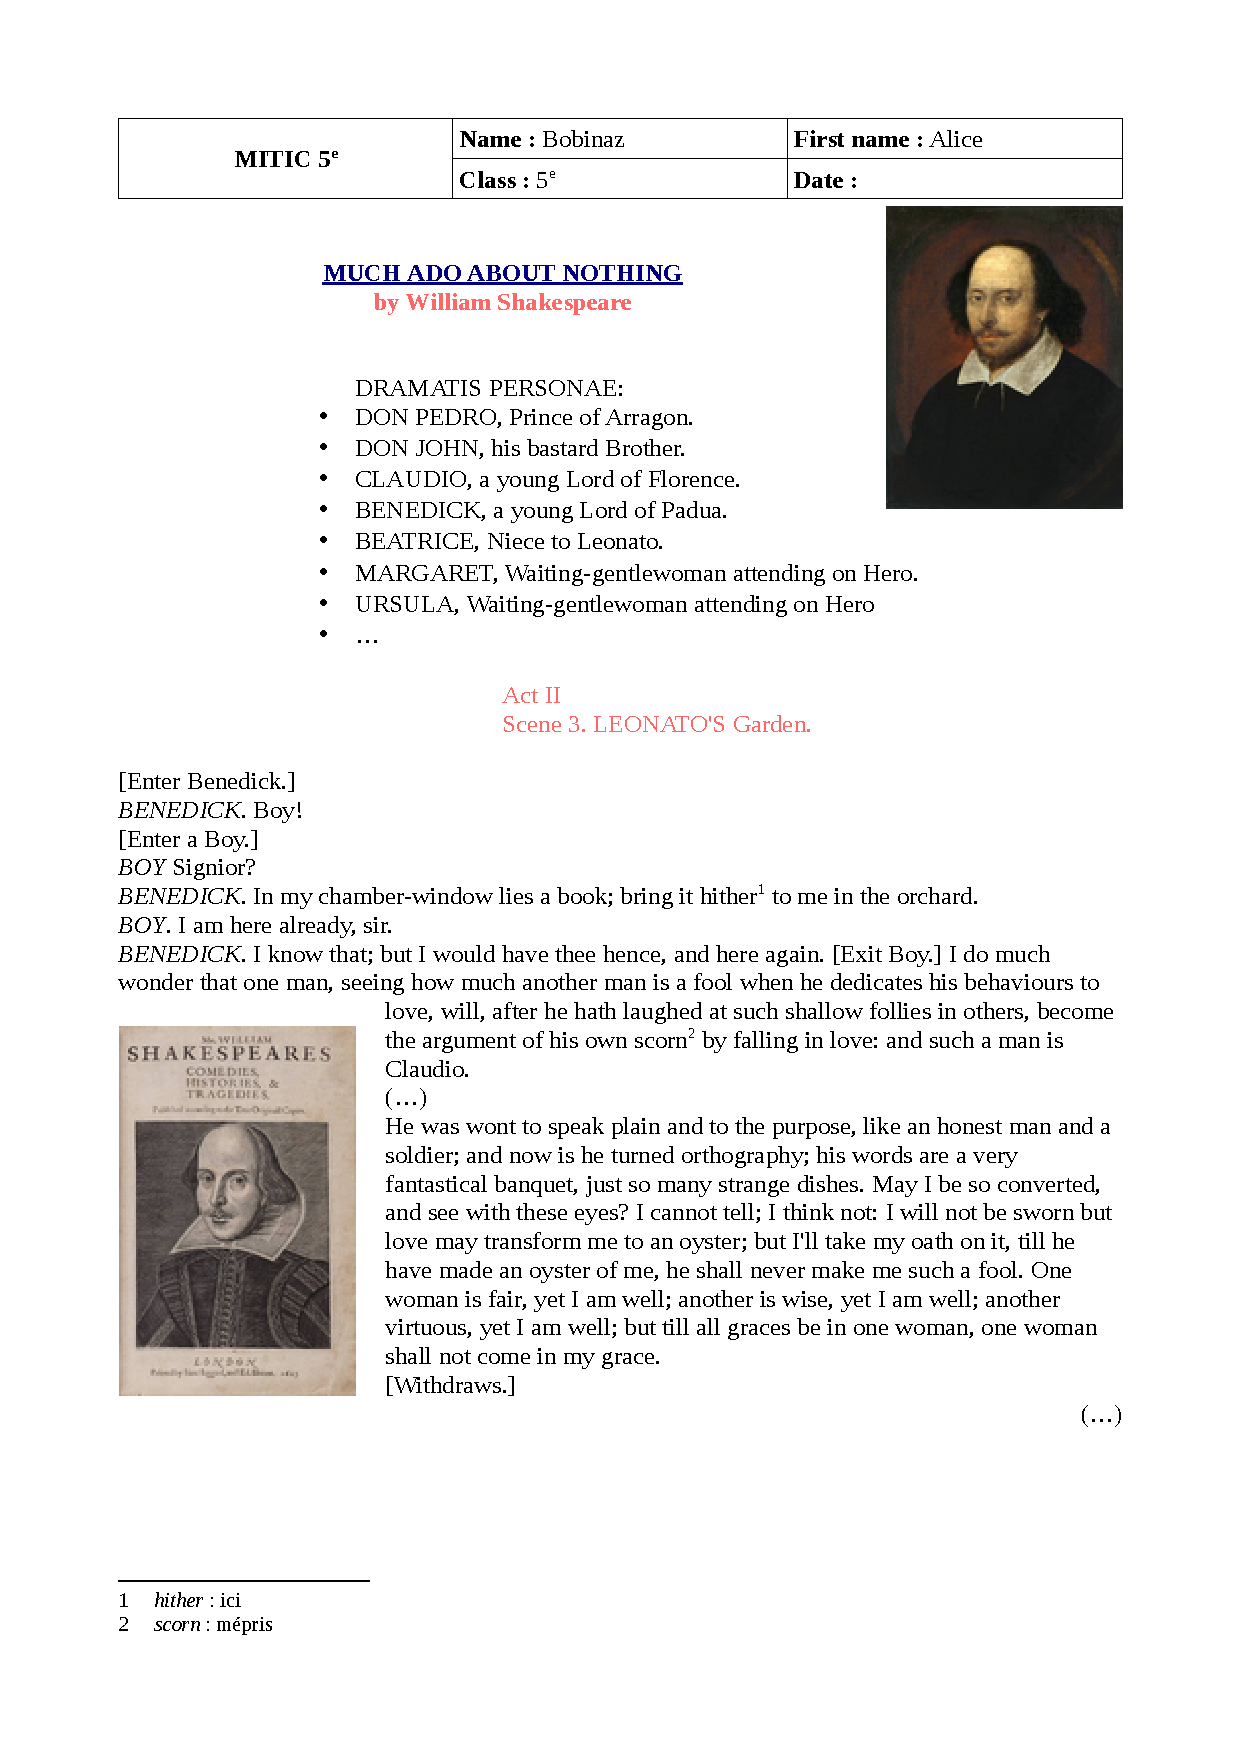
\includegraphics[width=.75\textwidth]{./sources/texte02/Shakespeare_MuchAdo_Formate}}\label{modelePage5e2}\end{center}

\textbf{Pour obtenir de l'aide, rendez-vous à la page \pageref{aide_seancesWord}}

\vfill
\phantom{rien}






%\cadre{Pensez à sauver régulièrement votre travail en appuyant sur \texttt{Cmd + s} ou à partir du menu \texttt{Fichier} en choisissant \texttt{Enregistrer}.

%\uneimageici{./images/generales/clavierCmdS}{.3\textwidth}
%}

%\newpage

%\phantom{rien}


%\vfill



%\vfill

%\phantom{rien} 







%
%
%  S  É  A  N  C  E     III
%
%

\newpage

\section{Séance 3 : mise en forme d'une fiche historique}\label{ficheTexte5e3}

\subsection{Pour bien démarrer...}

Dès que vous avez ouvert un nouveau document dans \emph{Word}, sauvegardez-le au format Nom-date.docx : dans le menu \texttt{Fichier}, choisir \texttt{Enregistrer}. Pendant que vous travaillez, pensez à sauvegarder régulièrement votre travail (raccourci clavier \texttt{Cmd + s}).   

\uneimageici{./images/generales/clavierCmdS}{.4\textwidth}

\subsection{L'activité demandée}

%\vspace{10pt}

\boiteEnonceLarge{Le but de cette séance est de mettre en forme une fiche historique, à partir de données récupérées sur un site internet. Le modèle à obtenir est montré page ci-dessous. Pour parvenir à ce résultat, vous devrez effectuer les étapes suivantes :
\begin{enumerate}
\item Récupérer la version brute du document sur la page \emph{Teams} de votre cours.
\item Ajouter le tableau au début du document, et le compléter.
\item Mettre en forme la page (marges de 2,5\,cm en haut et en bas, de 1,5\,cm à gauche et à droite).
\item Mettre en forme le texte en police Arial, taille 9, interligne simple et justifié.
\item Mettre en forme le titre \emph{Soliman le Magnifique}, en gras, Arial 16, centré. À côté du titre, ajouter une note de bas de page citant la source du texte : \url{http://www.istanbulguide.net/istguide/people/connus/soliman.htm} en indiquant aussi la date de consultation (\emph{<<\,consulté le 14 juin 2017\,>>}).
\item Ajouter un lien hypertexte pour le titre "Soliman le magnifique" qui pointe vers la page Wikipédia de ce personnage : \url{https://fr.wikipedia.org/wiki/Soliman_le_Magnifique}.
\item Sur la page Wikipédia de Soliman le Magnifique, récupérer l'image : il faut alors faire un clic droit sur l'image, puis choisir \texttt{Enregistrer l'image sous...} dans le menu contextuel qui s'ouvre. Enregistrer l'image sur le \texttt{Bureau} de l'ordinateur afin de la retrouver facilement. Insérer et positionner l'image dans le texte. Réduire sa taille pour que l'ensemble tienne sur une page.
\item Adapter le contour de l'image pour que le texte reste autour de l'image. Introduire les espacements suivants : 0,5\,cm pour chacune des valeurs. 
\end{enumerate}
}
\newpage
\boiteEnonceLarge{
Une fois la mise en forme terminée, vous exporterez votre fichier au format PDF (le fichier doit être nommé à partir de votre nom : \texttt{Nom-date.pdf}), puis vous le rendrez sur \emph{Teams} à l'endroit indiqué par votre enseignant (si nécessaire, se reporter à la fiche méthode \emph{Remettre son devoir}, page \pageref{TeamsRemettreDevoir}).}





\begin{center}\fbox{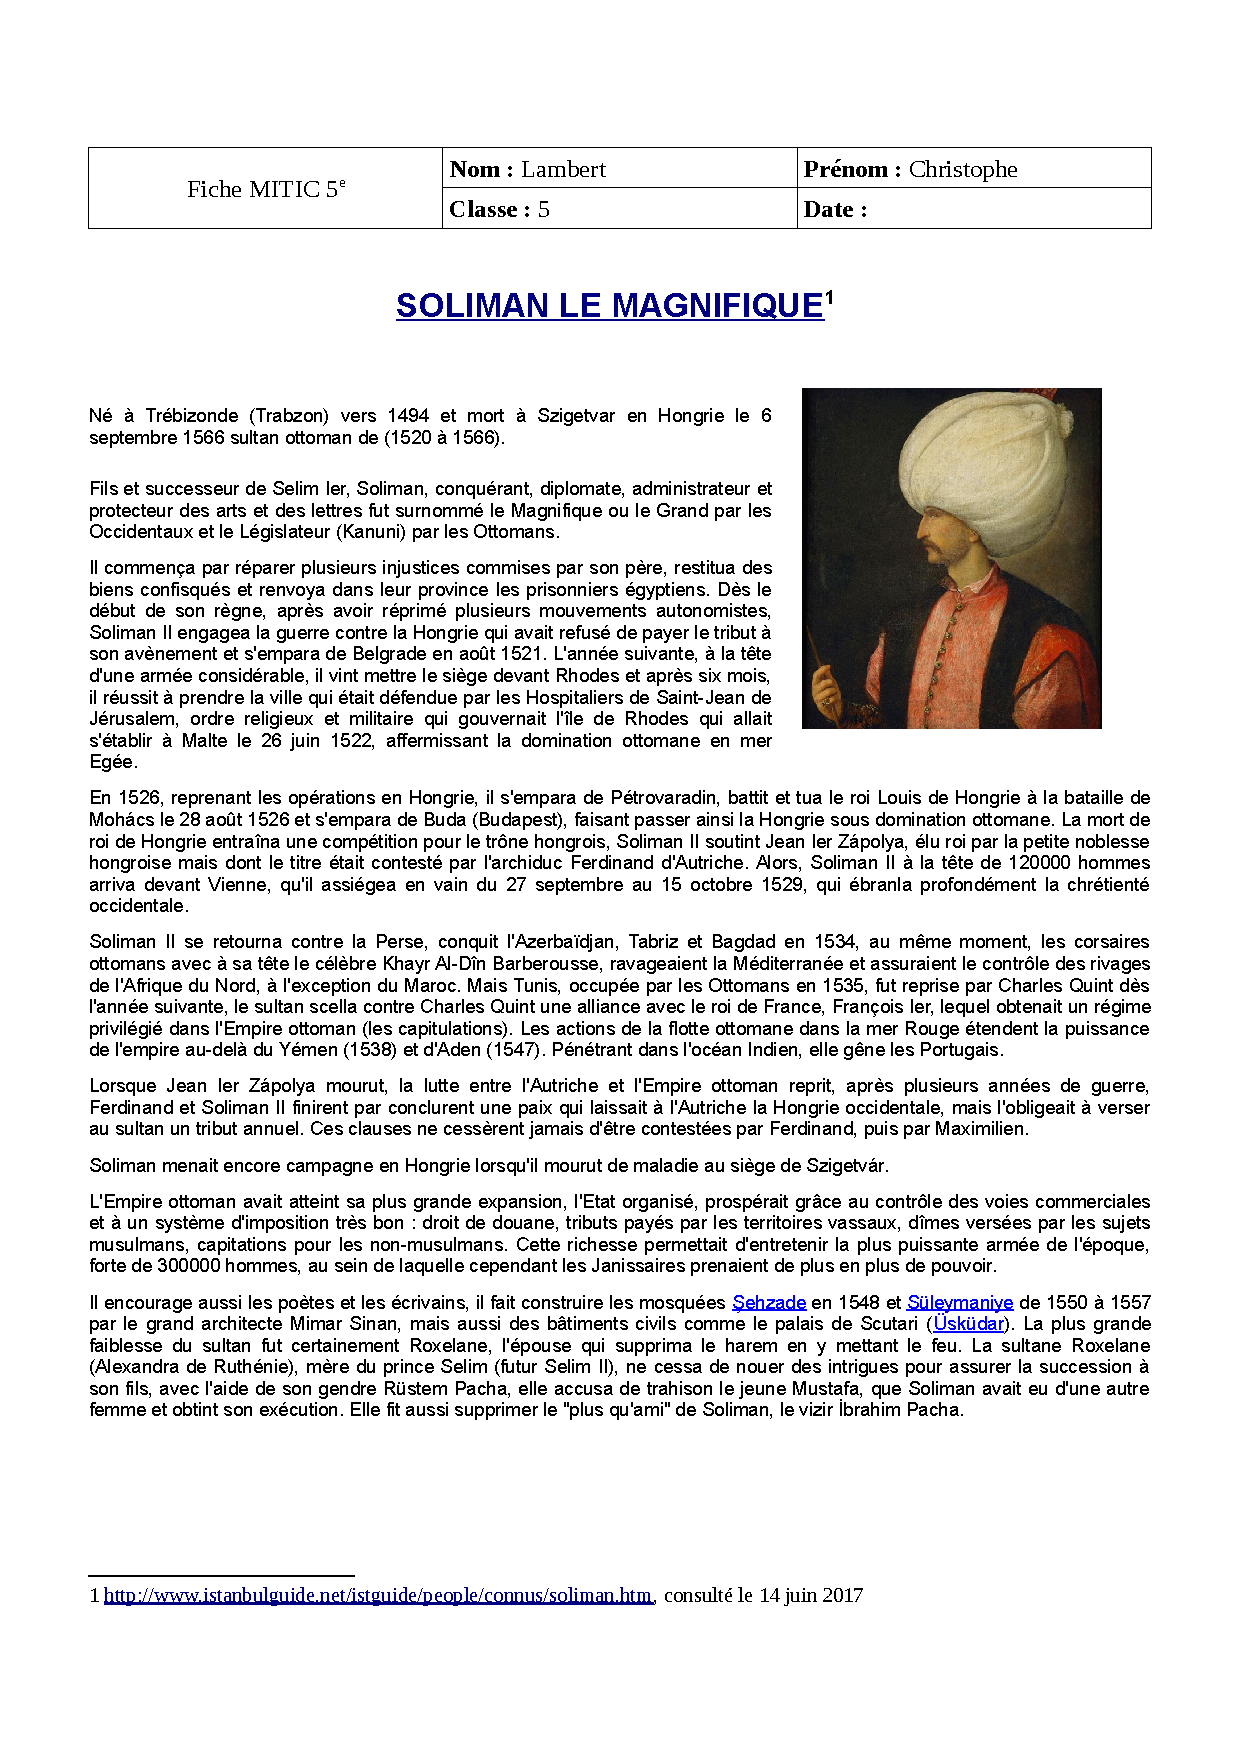
\includegraphics[width=.75\textwidth]{./sources/texte02/MiticHistoire5e}}\label{modelePage5e3}\end{center}

\textbf{Pour obtenir de l'aide, rendez-vous à la page \pageref{aide_seancesWord}}

\vfill
\phantom{rien}

%\cadre{Pensez à sauver régulièrement votre travail en appuyant sur \texttt{Cmd + s} ou à partir du menu \texttt{Fichier} en choisissant \texttt{Enregistrer}.

%\uneimageici{./images/generales/clavierCmdS}{.3\textwidth}
%}

%\newpage

%\phantom{rien}

%\vfill



%\phantom{rien} \vfill





%%%
% AIDE AUX ACTIVITES
%%%

\newpage

\section{Aide pour réaliser les activités}\label{aide_seancesWord}

%\section{Les outils dont vous aurez besoin}\label{Texte5eOutils}

Les nouveaux outils dont vous aurez besoin pour réaliser les trois séances sur le traitement de texte sont décrits ci-dessous :

%\hfill
\includegraphics[width=4cm]{./images/generales/NouvelOutil}

\begin{itemize}   
\item insérer un tableau, voir section \vref{Texte2InsererTableau} ;
\item créer une liste à puces, voir section \vref{Texte2ListePuce} ;
\item ajouter un lien hypertexte, voir section \vref{Texte2LienHyper} ;
\item insérer une note de bas de page, voir section \vref{Texte2NoteBasPage} ;
\item utiliser le correcteur d'orthographe, voir section \vref{Texte2CorrecteurOrtho} ;
\item insérer une image et adapter le texte autour de l'image, voir section \vref{Texte2InsererImage}.
\end{itemize}  



\subsection{Insérer un tableau}\index{Writer!Insérer un tableau}\index{Insérer un tableau (Writer)}\label{Texte2InsererTableau} 



Le but est de créer un tableau comme montré ci-dessous, que l'on pourra insérer par exemple en haut d'un document :

\uneimageici{./images/texte02/InsererTableauFini}{.8\textwidth}


Pour insérer un tableau, placer le curseur à la position où le tableau doit être inséré, puis dans le menu \texttt{Insérer}, choisir \texttt{Insérer un tableau}.\\ \emph{Remarque :} il est également possible d'utiliser directement l'icône \texttt{Ajouter un tableau} : 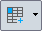
\includegraphics[width=.6cm]{./images/texte02/InsererTableauIcone}, ce qui produit le même effet.

  

\deuximagesGPici{./images/texte02/insererTableau1NEW.png}{\textwidth}%
                {./images/texte02/insererTableau2NEW.png}{.7\textwidth}  



Une boîte de dialogue s'ouvre alors (figure ci-dessous) : il faut choisir le nombre de colonnes et de lignes (par exemple ici un tableau de 5\,colonnes et 2\,lignes. On peut également choisir si la largeur initiale de chaque colonne s'adapte automatiquement à la largeur de la page ou si elle s'ajuste en fonction du contenu des colonnes. Terminer en cliquant sur le bouton \texttt{OK}.  

\uneimageici{./images/texte02/insererTableau3NEW}{.5\textwidth}

Un tableau vide est maintenant présent sur la page. Pour le remplir, il suffit de cliquer sur une cellule et d'y taper le texte souhaité.

\uneimageici{./images/texte02/InsererTableauVide}{.8\textwidth}

Pour fusionner deux cellules, il faut les sélectionner à l'aide de la souris :

\uneimageici{./images/texte02/InsererTableauSelection}{.8\textwidth}

Puis dans le menu \texttt{Tableau}, choisir \texttt{Fusionner les cellules}. \emph{Remarque :} il est également possible de faire un clic droit à l'aide de la souris sur les cases sélectionnées, et de choisir dans le menu qui s'ouvre \texttt{Fusionner} (figure à droite ci-dessous).  

\deuximagesGPici{./images/texte02/InsererTableauFusion}{\textwidth}%
                {./images/texte02/InsererTableauFusionSouris}{.9\textwidth}  




On peut alors compléter le texte dans la nouvelle cellule créée pour terminer le tableau :

\uneimageici{./images/texte02/InsererTableauFini}{.8\textwidth}

\vspace{24pt}



Remarque : pour centrer verticalement le texte <<\,\emph{Fiche MITIC 5\up{e}}\,>> dans la cellule\index{Writer!Tableau, centrer le contenu d'une cellule}\index{Tableau, centrer le contenu d'une cellule (Writer)}, deux solutions sont possibles :

\begin{itemize}
\item Sélectionner la cellule du tableau, faire un clic droit et choisir \texttt{Alignement}, puis \texttt{Centre}.  

\uneimageici{./images/texte02/InsererTableauCentrage}{.6\textwidth}

\item Utiliser directement l'icône de centrage du contenu d'une cellule 
\includegraphics[width=.6cm]{./images/texte02/iconeTableauCentrage} qui est situé dans la barre d'icône en bas de l'écran.
\end{itemize}  

\vspace{24pt} 

Pour supprimer un tableau\index{Writer!Tableau, supprimer le tableau}\index{Tableau, supprimer le tableau (Writer)} , il faut sélectionner à l'aide de la souris toutes les cellules qu'il contient, puis dans le menu \texttt{Tableau}, choisir \texttt{Supprimer} puis \texttt{Tableau}. Il est également possible de cette façon de supprimer des lignes ou des colonnes du tableau :

\uneimageici{./images/texte02/InsererTableauSupprimer}{.7\textwidth}







\subsection{Créer une liste à puces}\index{Writer!Liste à puces}\index{Liste à puces (Writer)}\label{Texte2ListePuce} 

La première étape consiste à écrire le texte, puis à sélectionner la partie qui doit être mise sous forme de liste à puces. Il faut alors se rendre dans le menu \texttt{Format}, puis choisir \texttt{Listes} et enfin \texttt{(Dés)activer les puces} :      

\uneimageici{./images/texte02/listePuces01}{.7\textwidth}

Il est possible également d'utiliser le bouton \texttt{(Dés)activer les puces} 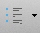
\includegraphics[width=.6cm]{./images/texte02/listePucesIcone}, ce qui produit le même effet :

\uneimageici{./images/texte02/listePuces02}{.7\textwidth}

Une fois la liste à puces obtenue, un retour à la ligne va créer une nouvelle puce :

\uneimageici{./images/texte02/listePuces03}{.4\textwidth}

Pour la faire disparaître, trois solutions :
\begin{itemize}
\item appuyer à nouveau sur la touche entrée ;
\item cliquer à nouveau sur le bouton \texttt{(Dés)activer les puces} 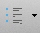
\includegraphics[width=.6cm]{./images/texte02/listePucesIcone} ;
\item appuyer deux fois sur la touche \texttt{Delete} :

\uneimageici{./images/generales/clavierDelete}{.3\textwidth}
\end{itemize}






\subsection{Ajouter un lien hypertexte}\index{Writer!Lien hypertexte}\index{Lien hypertexte (Writer)}\label{Texte2LienHyper}

Un \emph{lien hypertexte} permet de créer un groupe de mots sur lequel on peut cliquer et qui renvoie vers un site internet. Pour créer un lien hypertexte, il faut tout d'abord sélectionner le ou les mots sur lesquels on pourra cliquer, puis se rendre dans le menu \texttt{Insertion} et choisir \texttt{Hyperlien...} :    

\uneimageici{./images/texte02/Hyperlien1}{.6\textwidth}

Dans la boîte de dialogue qui s'ouvre, compléter le champ \texttt{Cible} en indiquant l'adresse internet complète du site qui doit être ouvert lorsque l'utilisateur clique sur le lien hypertexte (ici c'est le site \texttt{Wiktionnaire}\footnote{Le site \emph{Wiktionnaire} permet d'obtenir facilement la définition d'un mot. Il faut pour cela entrer comme lien l'adresse \texttt{https://fr.wiktionary.org/wiki/votreMot}, où \texttt{"votreMot"} est à remplacer par le mot dont on veut la définition.} qui est utilisé) :   

\uneimageici{./images/texte02/Hyperlien2}{.8\textwidth}

Le résultat est présenté ci-dessous. Le lien hypertexte apparaît mis en évidence, et si l'utilisateur clique sur le lien, il est alors dirigé vers le site internet choisi :

\uneimageici{./images/texte02/Hyperlien3}{.3\textwidth}




\subsection{Insérer une note de bas de page}\index{Writer!Note de bas de page}\index{Note de bas de page (Writer)}\label{Texte2NoteBasPage}

Lorsqu'on compose un texte, il est souvent utile d'ajouter une \emph{note de bas de page}\footnote{Une \emph{note de bas de page}, comme son nom l'indique, est un petit texte qui se situe au niveau du pied de page et qui permet d'ajouter une définition, un commentaire ou une référence à une partie de texte.}.

Pour introduire une note de bas de page, placer le curseur à la suite du mot où la note doit apparaître. Dans le menu \texttt{Insertion}, choisir alors \texttt{Note de bas de page / de fin}, puis \texttt{Note de bas de page}.       

\uneimageici{./images/texte02/InsererNoteBasPage1}{.5\textwidth}

Le curseur se positionne alors dans le pied de page afin que le texte correspondant à la note de bas de page soit entré, comme montré sur la figure ci-dessous.

\uneimageici{./images/texte02/InsererNoteBasPage2}{.8\textwidth}

Le traitement de texte gère tout seul la numérotation des notes de bas de page ainsi que leur position dans le document.




\subsection{Utiliser le correcteur d'orthographe}\index{Writer!Correcteur d'orthographe}\index{Correcteur d'orthographe (Writer)}\label{Texte2CorrecteurOrtho}

Pour pouvoir utiliser les fonctionnalités de correction orthographique, il faut tout d'abord choisir une langue pour le texte. Ceci est possible en cliquant sur le menu \texttt{Outils}, choisir \texttt{Langue} puis \texttt{Pour tout le texte} et enfin \texttt{Français (France)} :

\uneimageici{./images/texte02/Correction0}{.8\textwidth}

Une fois cette sélection effectuée, les mots non reconnus apparaissent soulignés en rouge, comme montré sur la figure suivante :

\uneimageici{./images/texte02/Correction1}{.4\textwidth}

Pour corriger le mot, il faut faire un clic droit sur le mot souligné. Un menu s'ouvre alors et propose différentes corrections possibles. Il suffit de choisir une des corrections proposées :

\uneimageici{./images/texte02/Correction2}{.4\textwidth}

\emph{Remarque :} comme montré sur la figure précédente, il est également possible d'ignorer une erreur (choisir \texttt{Ignorer}) ou d'ajouter un mot au dictionnaire pour qu'il soit reconnu comme correct (choisir \texttt{Ajouter au dictionnaire}).    




\subsection{Insérer une image et adapter le texte autour de l'image}\index{Writer!Image, adapter le texte}\index{Image, adapter le texte (Writer)}\label{Texte2InsererImage}

Pour insérer une image, placer le curseur à l'endroit où l'image doit être insérée. Dans le menu \texttt{Insertion} choisir alors \texttt{Insérer une image...} Il est également possible d'utiliser directement l'icône 
\includegraphics[width=.6cm]{./images/texte02/iconeInsererImage}. 

\deuximagesici{./images/texte02/InsererImage1}{\textwidth}%
              {./images/texte02/InsererImage2}{\textwidth}

L'image insérée peut être déplacée en utilisant la souris : le pointeur se transforme alors en une main 
\includegraphics[width=.3cm]{./images/texte02/pointeurMain} qui permet de faire glisser l'image (observez la petite ancre 
\includegraphics[width=.4cm]{./images/texte02/iconeAncre} qui se déplace avec l'image).



Pour régler la taille de l'image, deux solutions :
\begin{itemize}
\item effectuer un double-clic sur l'image ;
\item effectuer un clic droit sur l'image et choisir dans le menu contextuel \texttt{Formater l'image...}  
\end{itemize}

Dans la boîte de dialogue qui s'ouvre alors, choisir l'onglet \texttt{Type} et définir sa largeur ou sa hauteur (sans oublier de cocher \texttt{Conserver le ratio}, sinon l'image va être déformée !). 

\uneimageici{./images/texte02/InsererImage5}{.8\textwidth}

L'onglet \texttt{Adapter} permet de définir comment le texte va s'\emph{adapter} à l'image, c'est-à-dire comment il sera disposé autour de l'image (\circled{1} sur la figure ci-dessous). On peut également définir la distance qui sépare le texte de l'image \circled{2}.  

\uneimageici{./images/texte02/InsererImage6}{.8\textwidth}

Sur la figure ci-dessous, le texte est adapté en \emph{parallèle} autour de l'image : 

\uneimageici{./images/texte02/InsererImage7}{.5\textwidth}





\emph{Remarque :} un clic droit sur l'image permet d'ouvrir un menu contextuel qui propose un accès direct à la plupart des réglages de l'image (figure ci-dessous). 

\uneimageici{./images/texte02/InsererImage3}{.7\textwidth}







\chapter{Traitement d'images}  

Un logiciel de traitement d'images est un logiciel qui permet d'effectuer des modifications sur une image existante : taille de l'image, luminosité, contraste, recadrage, etc...\\

{\footnotesize
\begin{itemize}
\item Logiciel\footnote{Le logiciel Gimp est librement téléchargeable : \url{http://www.gimp.org/}} : \emph{Gimp}
\item Prérequis (se reporter si nécessaire aux \emph{Fiches MITIC 6\up{e}}) :
        \begin{itemize}
        \item recadrer une image ;
        \item exporter une image dans un autre format ;
        \item ajouter un cadre autour d'une image ;
        \item régler la luminosité et le contraste.
        \end{itemize}
\item Matières concernées : français et arts visuels.
\item Compétences : 
        \begin{itemize}
        \item ajouter un texte sur une image et le mettre en forme ;
        \item appliquer un filtre sur une portion de l'image ;
        \item convertir une image en niveaux de gris ;
        \item réaliser une copie d'écran ;
        \item utiliser les calques.
        \end{itemize}
\item Cette fiche est à réaliser :
        \begin{itemize}
        \item avant les vacances d'été en français (séance 1) ;
        \item avant la fin du semestre de cours en arts visuels (séance 2).
        \end{itemize}
\end{itemize}
} % fin du footnotesize

\vspace{12pt}

Les compétences listées ci-dessous ont été vues en classe de 6\up{e}. Vous en aurez à nouveau besoin pour les activités de cette année. Si nécessaire, reportez-vous aux \emph{Fiches MITIC 6\up{e}} pour revoir comment :  

\begin{itemize}
\item recadrer une image ;
\item exporter une image dans un autre format ;
\item ajouter un cadre autour d'une image en changeant la taille du canevas ;
\item régler la luminosité et le contraste.
\end{itemize}









\newpage

%
%
%  S  É  A  N  C  E     I
%
%


\section{Séance 1 : un haïku écrit sur une image}\label{ficheImage5e1}


\subsection{Pour bien démarrer...}

Lorsque la fenêtre principale du logiciel s'ouvre, elle devrait ressembler à cela :

\uneimageici{./images/image02/GimpInterface}{.7\textwidth}

Si ce n'est pas le cas, alors il faut effectuer les réglages suivants :

\begin{minipage}[c]{.58\textwidth}
\begin{itemize}
\item Ouvrir le menu \texttt{Fenêtre}, puis cocher la case \texttt{Mode fenêtre unique}.
\item Dans le même menu, cliquer également sur \texttt{Boîte à outils} pour faire apparaître les outils.
\end{itemize}
\end{minipage}\hfill%
\begin{minipage}[c]{.38\textwidth}
\uneimageici{./images/image02/GimpMenuFenetre2}{.9\textwidth}
\end{minipage}

Toutefois, si la couleur de l'interface est plus claire ou si la barre d'outils est un peu différente ou positionnée différemment, ce n'est pas grave : l'essentiel est de retrouver les différentes icônes qui elles, sont les mêmes.

\subsection{Pensez à enregistrer régulièrement}

Dès que vous avez ouvert un nouveau fichier dans \emph{Gimp}, sauvegardez-le au format Nom-date.png : dans le menu \texttt{Fichier}, choisir \texttt{Enregistrer}. Pendant que vous travaillez, pensez à sauvegarder régulièrement votre travail (raccourci clavier \texttt{Cmd + s}).   

\uneimageici{./images/generales/clavierCmdS}{.4\textwidth}

\vfill
\phantom{rien}
%\vspace{10pt}

\subsection{L'activité demandée}

\vspace{10pt}

\boiteEnonceLarge{Le but de cette séance est d'écrire un haïku sur une image, comme le montre l'exemple ci-dessous (haïku écrit par \emph{Bash\={o} Matsuo}, un des quatre maîtres classiques de la discipline). Un \emph{haïku} est un poème très court dont le but est de dire et de célébrer l'évanescence des choses\footnote{D'après la définition donnée sur la page Wikipedia du haïku.}. Ce type de poème a été inventé au Japon au XVIIe siècle.
\vspace{5pt}

%
%\begin{minipage}[c]{.48\textwidth}
%\centering%
\includegraphics[angle=0,width=.3\textwidth]{./images/image02/haiku}
%\end{minipage}
% 
\vspace{5pt}

Pour parvenir à ce résultat, vous devrez effectuer les étapes suivantes :
\begin{enumerate}
\item Écrire un poème de type haïku de votre choix.
\item Se rendre sur le site d'images librement utilisables \url{https://www.pexels.com} et choisir une image pour illustrer votre poème. La télécharger en taille \emph{medium} (l'enregistrer sur le \emph{Bureau} de l'ordinateur pour la retrouver facilement). Ce site est une bibliothèque d'images sous \emph{licence libre} qu'il est donc possible d'utiliser et de modifier librement\footnote{Pour obtenir davantage d'informations sur les licences libres, se rendre sur le site de \emph{Creative Commons} \url{https://creativecommons.fr/}.}.
\item Ouvrir l'image à l'aide du logiciel Gimp. Si une boîte de dialogue s'ouvre pour vous proposez de convertir le profil de couleur de l'image, cliquer sur \texttt{Convertir}.
\item Si nécessaire, recadrer l'image ou convertir l'image en niveaux de gris.
\item Sélectionner une zone de l'image (là où vous allez écrire le poème) et ajouter un flou gaussien (menu \texttt{Filtre}, choisir \texttt{Flou} puis \texttt{Flou gaussien}).   
\item La zone étant toujours sélectionnée, augmenter la luminosité afin d'éclaircir l'image à cet endroit (menu \texttt{Couleurs}, choisir \texttt{Luminosité-Contraste}). 
\item Ajouter alors le texte du poème et régler la police de caractères, la couleur et la taille des caractères. Positionner le texte à l'endroit de votre choix.
\item Pour aller plus loin (facultatif), ajouter un cadre autour de l'image.
\end{enumerate}
Une fois le travail terminé, vous exporterez l'image au format PNG (le fichier doit être nommé à partir de votre nom : \texttt{Nom-date.png}), puis vous le rendrez sur \emph{Teams} à l'endroit indiqué par votre enseignant (si nécessaire, se reporter à la fiche méthode \emph{Remettre son devoir}, page \pageref{TeamsRemettreDevoir}).}
% fin de l'énoncé

%\vfill
%\phantom{rien}

%\begin{minipage}[c]{.48\textwidth}
%L'objectif est d'obtenir une image comme par exemple celle montrée ci-dessous 
%\end{minipage}\hfill%


%\vfill
%\phantom{rien}




%
%
%  S  É  A  N  C  E     II
%
%


\section{Séance 2 : superposition d'images}\label{ficheImage5e2}

\subsection{Pour bien démarrer...}

Dès que vous avez ouvert un nouveau fichier dans \emph{Gimp}, sauvegardez-le au format Nom-date.png : dans le menu \texttt{Fichier}, choisir \texttt{Enregistrer}. Pendant que vous travaillez, pensez à sauvegarder régulièrement votre travail (raccourci clavier \texttt{Cmd + s}).   

\uneimageici{./images/generales/clavierCmdS}{.4\textwidth}

%\vspace{10pt}

%\vfill
%\phantom{rien}

\subsection{L'activité demandée}

\vspace{10pt}

\boiteEnonceLarge{Le but de cette séance est de superposer des images et d'utiliser les réglages d'opacité des calques afin d'en obtenir une nouvelle, comme le montre l'exemple ci-dessous (à gauche les trois images de base utilisées et à droite l'image finale obtenue).\\ 

\begin{minipage}[c]{.38\textwidth}
\begin{center}
\includegraphics[angle=0,width=.4\textwidth]{./sources/image02/seanceArts/01_Road}

\vspace{4pt}

\includegraphics[angle=0,width=.4\textwidth]{./sources/image02/seanceArts/02_Tower}

\vspace{4pt}

\includegraphics[angle=0,width=.4\textwidth]{./sources/image02/seanceArts/03_Tiger}
\end{center}
\end{minipage}\hfill%
\begin{minipage}[c]{.6\textwidth}
\centering%
\includegraphics[angle=0,width=.85\textwidth]{./sources/image02/seanceArts/seanceArts5e}
\end{minipage}
}
\vfill
\phantom{rien}
\boiteEnonceLarge{
Pour parvenir à ce résultat, vous devrez utiliser les outils présentés en début de chapitre (voir section \vref{Image5eOutils}).
\begin{enumerate}
\item Récupérer trois images de base sur la page Teams de votre cours.
\item Ouvrir une de ces images sous Gimp.
\item Créer deux nouveaux calques (leur donner un nom explicite) et y copier les deux autres images : vous devez alors avoir sous Gimp une image composée de trois calques qui contiennent chacun une image fournie par l'enseignant.
\item Choisir l'ordre des calques en utilisant les flèches \includegraphics[width=1cm]{./images/image02/CalqueOrdonner} situées en bas de la fenêtre des calques, afin que l'image utilisée comme arrière-plan apparaisse tout en bas de la pile de calque. Faire de même pour les deux autres images (les positionner au bon endroit). 
\item Régler l'opacité des deux calques du haut à 50\,\%\ afin de voir par transparence les trois images.  
\item À l'aide de l'outil de déplacement des calques \includegraphics[width=.4cm]{./images/image02/iconeDeplacement}, positionner chacune des images à l'endroit souhaité. Utiliser si nécessaire l'œil \includegraphics[width=.6cm]{./images/image02/iconeOeil} qui permet d'afficher ou non un calque.
\item Une fois le positionnement effectué, terminer de régler l'opacité des calques pour obtenir le résultat désiré.
\item Ajouter prénom et nom à l'aide de l'outil d'ajout de texte et effectuer sa mise en forme.
\item Pour aller plus loin (facultatif), ajouter un cadre autour de l'image.
\end{enumerate}
Une fois le travail terminé, vous exporterez l'image au format PNG (le fichier doit être nommé à partir de votre nom : \texttt{Nom-date.png}), puis vous le rendrez sur \emph{Teams} à l'endroit indiqué par votre enseignant (si nécessaire, se reporter à la fiche méthode \emph{Remettre son devoir}, page \pageref{TeamsRemettreDevoir}).}
% fin de l'énoncé





% AIDE

\newpage

\section{Aide pour réaliser les activités}\label{Image5eOutils}
 
Les nouveaux outils dont vous aurez besoin pour réaliser les deux séances sur le traitement d'images sont décrits ci-dessous :

\begin{itemize}   
\item ajouter un texte sur une image, voir section \vref{Gimp2AjouterTexte} ;
\item ajouter un filtre sur une portion de l'image, voir section \vref{Gimp2AppliquerFiltre} ;
\item convertir une image en noir et blanc (niveaux de gris), voir section \vref{Gimp2ConvertirNoirBlanc} ;
\item travailler avec les calques, voir section \vref{Gimp2Calques} ;   
\item réaliser une capture d'écran, voir section \vref{CaptureEcran2}.
\end{itemize}  



\subsection{Ajouter un texte}\index{Gimp!Ajouter un texte sur une image}\index{Ajouter un texte sur une image (Gimp)}\label{Gimp2AjouterTexte}

Pour ajouter un texte sur une image, il faut utiliser l'\texttt{outil texte} \includegraphics[width=.6cm]{./images/image02/iconeTexte} :

\uneimageici{./images/image02/TexteSurImage1}{.6\textwidth}

Il faut ensuite cliquer approximativement à l'endroit où l'on souhaite ajouter le texte, ce qui a pour effet d'ouvrir une petite boîte de dialogue contenant les outils pour mettre en forme le texte :

\uneimageici{./images/image02/TexteSurImage2}{.6\textwidth}

Taper le texte, le mettre en forme. Remarque : pour appliquer une mise en forme une fois le texte tapé, il faut comme d'habitude le sélectionner avant à l'aide de la souris.

\uneimageici{./images/image02/TexteSurImage3}{.6\textwidth}

Remarque importante\label{remarqueCalque} : lorsque l'on ajoute un texte sur une image, un nouveau \emph{calque} est créé, comme on peut le voir dans la fenêtre des calques\index{Gimp!Calques}\index{Calques (Gimp)}. Sur la figure ci-dessous, la fenêtre des calques est active comme le montre l'onglet calque \circled{1}, et le calque actif est celui qui contient le texte \circled{2}. Avant de modifier ou déplacer le texte, il faut bien vérifier que le calque texte est actif. Si ce n'est pas le cas, il suffit de cliquer dessus, dans la fenêtre des calques. Pour plus d'information sur les calques, se reporter à la section \vref{Gimp2Calques}. 

\uneimageici{./images/image02/TexteSurImage4}{.3\textwidth}

Pour déplacer le texte, on utilise l'\texttt{outil de déplacement} \includegraphics[width=.6cm]{./images/image02/iconeDeplace}. Il faut alors positionner la souris sur le texte et chercher la bonne position pour que le curseur apparaisse sous cette forme : \includegraphics[width=.6cm]{./images/image02/iconeTexteBouge}. Observez bien les deux images ci-dessous : à gauche on ne peut pas déplacer le texte car le curseur n'a pas la bonne forme, par contre à droite il est possible de déplacer le texte.


\begin{minipage}[c]{.46\textwidth}
\centering%
\includegraphics[angle=0,width=.4\textwidth]{./images/image02/TexteCurseurBougePas}
\end{minipage}\hfill%
\begin{minipage}[c]{.46\textwidth}
\centering%
\includegraphics[angle=0,width=.4\textwidth]{./images/image02/TexteCurseurBouge}
\end{minipage}\\[12pt]
\begin{minipage}[c]{.46\textwidth}
{\small \emph{Avec un curseur de cette forme, c'est le calque qui se déplace.}}
\end{minipage}\hfill%
\begin{minipage}[c]{.46\textwidth}
{\small \emph{Avec un curseur de cette forme, c'est le texte qui se déplace.}}
\end{minipage}

\vspace{1em}

\textbf{Remarque :} on peut déplacer le texte directement sans chercher la bonne position en se plaçant sur le texte et en maintenant la touche \texttt{Shift} enfoncée.



\subsection{Appliquer un filtre sur une portion de l'image}\index{Gimp!Appliquer un filtre}\index{Appliquer un filtre (Gimp)}\label{Gimp2AppliquerFiltre}

Nous allons flouter un visage pour montrer l'usage d'un filtre sur une portion de l'image.

Pour cela, il faut sélectionner la partie souhaitée à l'aide d'un des outils de sélection. On peut sélectionner une zone rectangulaire \includegraphics[width=.6cm]{./images/image02/iconeSelecRectangle}, une zone ovale \includegraphics[width=.6cm]{./images/image02/iconeSelecOvale} ou sélectionner une zone <<\,à main levée\,>> \includegraphics[width=.6cm]{./images/image02/iconeSelecLasso}.

\vspace{6pt}

Attention, si un texte a été ajouté auparavant sur l'image, il faut se repositionner sur le calque correspondant à l'image (se reporter si nécessaire à la section \vref{Gimp2Calques}). 

\vspace{6pt}

Sur la figure ci-dessous, le visage a été sélectionné à l'aide de l'outil de sélection ovale.

\uneimageici{./images/image02/FiltrePixel1}{.55\textwidth}

Une fois la zone sélectionnée, dans le menu \texttt{Filtres}, choisir \texttt{Flou}, puis \texttt{Pixéliser...}   

\uneimageici{./images/image02/FiltrePixel2}{.6\textwidth}

Dans la boîte de dialogue qui s'ouvre alors (figure à gauche ci-dessous), modifier les paramètres afin d'obtenir le résultat souhaité puis cliquer sur le bouton \texttt{OK}. Le résultat obtenu est montré sur la figure de droite ci-dessous.

\deuximagesici{./images/image02/FiltrePixel3}{.6\textwidth}%
              {./images/image02/FiltrePixel4}{.6\textwidth}




\subsection{Convertir une image en noir et blanc}\index{Gimp!Convertir en niveaux de gris}\index{Convertir en niveaux de gris (Gimp)}\label{Gimp2ConvertirNoirBlanc}

 Pour convertir une image couleur en noir et blanc (le terme exact est en \emph{niveaux de gris}), il faut, dans le menu \texttt{Image}, choisir \texttt{Mode} puis \texttt{Niveaux de gris}. L'image est immédiatement convertie. Remarque : on peut également faire directement un clic droit sur l'image (comme montré sur la figure ci-dessous), puis choisir \texttt{Image}, \texttt{Mode} et \texttt{Niveaux de gris}.

\deuximagesGPici{./images/image02/NoirBlanc1}{\textwidth}%
              {./images/image02/NoirBlanc2}{.6\textwidth}




\subsection{Travailler avec les calques}\label{Gimp2Calques}\index{Calques}\index{Gimp!Calques}

Dans Gimp il est possible de travailler avec des \emph{calques} qui correspondent à des couches successives que l'on ajoute sur l'image de base. L'image finale correspond alors à la superposition de tous les calques. Toute la gestion des calques se passe dans la fenêtre des calques.

\vspace{6pt}

Observez l'exemple ci-dessous : l'image de droite est composée de trois calques, représentés séparément à gauche.

\vspace{12pt}

\begin{minipage}[c]{.22\textwidth}
\centering%
\fbox{\includegraphics[angle=0,width=.7\textwidth]{./images/image02/exempleCalquesVitraux}}
\end{minipage}\hfill%
\begin{minipage}[c]{.22\textwidth}
\centering%
\fbox{\includegraphics[angle=0,width=.7\textwidth]{./images/image02/exempleCalquesFleur}}
\end{minipage}\hfill%
\begin{minipage}[c]{.22\textwidth}
\centering%
\fbox{\includegraphics[angle=0,width=.7\textwidth]{./images/image02/exempleCalquesCinq}}
\end{minipage}\hfill%
\begin{minipage}[c]{.22\textwidth}
\centering%
\fbox{\includegraphics[angle=0,width=.7\textwidth]{./images/image02/exempleCalques}}
\end{minipage}\\[12pt]
\begin{minipage}[c]{.22\textwidth}
\centering {\footnotesize Calque 1 : le fond.}
\end{minipage}\hfill%
\begin{minipage}[c]{.22\textwidth}
\centering {\footnotesize Calque 2 : la fleur.}
\end{minipage}\hfill%
\begin{minipage}[c]{.22\textwidth}
\centering {\footnotesize Calque 3 : le 5.}
\end{minipage}\hfill%
\begin{minipage}[c]{.22\textwidth}
\centering {\footnotesize L'image finale.}
\end{minipage}


\vspace{12pt}

La figure ci-dessous montre la fenêtre des calques correspondant à l'image ci-dessus : on y retrouve bien les trois calques correspondant à chacune des couches. Attention, l'ordre des calques est très important : le calque le plus haut de la pile cache les autres (ici la fleur est au-dessus du fond et le 5 est au-dessus de la fleur et du fond).

\uneimageici{./images/image02/CalqueFenetre}{.4\textwidth}





\subsubsection{Ajouter un calque}\label{Gimp2CalquesAjouter}\index{Calques : ajouter}\index{Gimp!Ajouter un calque}

Pour ajouter un calque, il faut se rendre dans la fenêtre des calques et cliquer sur l'icône \includegraphics[width=.4cm]{./images/image02/CalqueAjouter} (figure ci-dessous à gauche). Une boîte de dialogue s'ouvre alors (figure ci-dessous au centre) : elle permet de choisir le nom du calque (que l'on peut modifier par la suite en double-cliquant sur celui-ci) et le type de remplissage (choisir \texttt{Transparence}). Le nouveau calque apparaît alors dans la fenêtre des calques (figure ci-dessous à droite).

\vspace{12pt}

\begin{minipage}[c]{.32\textwidth}
\centering%
\includegraphics[angle=0,width=.85\textwidth]{./images/image02/GimpCalqueAjouter1}
\end{minipage}\hfill%
\begin{minipage}[c]{.32\textwidth}
\centering%
\includegraphics[angle=0,width=.85\textwidth]{./images/image02/GimpCalqueAjouter2}
\end{minipage}\hfill%
\begin{minipage}[c]{.32\textwidth}
\centering%
\includegraphics[angle=0,width=.85\textwidth]{./images/image02/GimpCalqueAjouter3}
\end{minipage}

\vspace{12pt}

Remarque importante : le \emph{calque actif}\index{Calques : changer de calque actif}\index{Gimp!Changer de calque actif}, c'est-à-dire le calque sur lequel on est en train de travailler, apparaît coloré dans la fenêtre des calques.


\subsubsection{Modifier l'opacité d'un calque}\label{Gimp2CalquesOpacite}\index{Calques : modifier l'opacité}\index{Gimp!Modifier l'opacité d'un calque} 

\emph{Modifier l'opacité} d'un calque signifie le rendre plus ou moins transparent afin que l'on puisse <<\,voir à travers\,>>.

Pour modifier l'opacité d'un calque, il suffit de le rendre actif en cliquant dessus dans la fenêtre des calques, puis de modifier la valeur de l'opacité à l'aide du curseur \texttt{Opacité} \includegraphics[width=3.5cm]{./images/image02/BarreOpacite}. Si le calque est opaque à 100\,\%\ alors on ne voit pas les calques situés au-dessous. Si le calque a une opacité de 0\,\%\, alors il n'est plus visible. Pour rendre invisible un calque, il est également possible de cliquer sur l'œil \includegraphics[width=.6cm]{./images/image02/iconeOeil} dans la fenêtre des calques.

Sur la figure ci-dessous, le calque contenant la fleur a une opacité de 70\,\% : on voit donc le fond par transparence à travers la fleur.  

\uneimageici{./images/image02/GimpCalqueOpacite2}{.55\textwidth}



\subsubsection{Modifier la pile des calques}\label{Gimp2CalquesOrdonner}\index{Calques : modifier la pile des calques}\index{Gimp!Modifier la pile des calques}

Tous les calques sont empilés les uns sur les autres. Le calque le plus bas dans la pile est recouvert par tous les autres. Il est parfois nécessaire de modifier la position d'un calque dans la pile des calques. Pour cela, deux solutions sont possibles :
\begin{itemize}
\item déplacer simplement le calque dans la fenêtre des calques à l'aide de la souris en effectuant un glisser-déposer ;
\item utiliser les boutons de déplacement du calque actif \includegraphics[width=1cm]{./images/image02/CalqueOrdonner} situés en bas de la fenêtre des calques.
\end{itemize}




\subsubsection{Déplacer un calque}\label{Gimp2CalquesDeplacer}\index{Calques : déplacer le calque}\index{Gimp!Déplacer un calque} 

À l'aide de l'outil de déplacement \includegraphics[width=.4cm]{./images/image02/iconeDeplacement} disponible dans la palette d'outils (figure ci-dessous à gauche), il est possible de déplacer le calque actif. Sur la figure à droite ci-dessous, le calque contenant la fleur (dont le contour est visible, en pointillés noir et jaune) est déplacé à l'aide de la souris. 

\deuximagesPGici{./images/image02/GimpCalqueDeplacer1}{.5\textwidth}%
              {./images/image02/GimpCalqueDeplacer2}{.9\textwidth}






\subsection{Réaliser une copie d'écran}\label{CaptureEcran2}\index{Capture d'écran}\index{Gimp!Capture d'écran}

Il est parfois nécessaire de copier le contenu de l'écran sous forme d'image pour pouvoir l'utiliser dans un document ou une présentation.

\vspace{12pt}

Pour réaliser une copie d'écran :

\begin{enumerate}
\item Capturer l'écran en utilisant un des raccourcis clavier suivant :
        \begin{itemize}
        \item \texttt{Ctrl + Maj + Cmd + 3} pour copier la totalité de l'écran,\index{Raccourci Clavier! Ctrl + Maj + Cmd + 3, copier tout l'écran}
        \item \texttt{Ctrl + Maj + Cmd + 4} pour copier une partie de l'écran (à sélectionner à la souris) ;\index{Raccourci Clavier! Ctrl + Maj + Cmd + 4, copier une partie de l'écran}
        \end{itemize} 

\uneimageici{./images/generales/clavierCapEcran}{.6\textwidth}

\item Coller l'image dans un nouveau document sous \emph{Gimp} : 
\end{enumerate}

\uneimageici{./images/image02/GimpCollerCommeImage}{.6\textwidth}

On peut alors retravailler l'image comme vous l'avez appris dans cette fiche sur \emph{Gimp}. 


\chapter{Traitement du son}  

Le traitement du son a pour objectif d'améliorer la qualité de signaux au format audio, de les compresser ou encore d'en extraire une information. On distingue généralement les signaux analogiques représentés par des flux continus de données des signaux digitaux représentés par une séquence de symboles binaires.

{\footnotesize
\begin{itemize}
\item Logiciel\footnote{Le logiciel Audacity est librement téléchargeable : \url{http://www.audacityteam.org/}} : \emph{Audacity 2.0} 
\item Prérequis : aucun
\item Matières concernées : anglais.
\item Compétences : 
        \begin{itemize}
        \item passer une piste stéréo en mono ;
        \item ajouter une piste ;
        \item copier et coller une partie de piste ;
        \item déplacer une partie de piste (glissement temporel)
        \item rendre silencieuse une partie d'une piste ;
        \item supprimer et raccorder ;
        \item réaliser un fondu en ouverture ou en fermeture ;
        \item exporter un projet au format MP3 ou WAV.
        \end{itemize}
\item Cette fiche est à réaliser :
        \begin{itemize}
        \item avant les vacances de printemps en anglais (séance 1) ;
        %\item avant la fin du semestre de cours en musique (séance 2). 
        \end{itemize}
\end{itemize}
}% fin du footnotesize




Audacity est un enregistreur et éditeur audio libre et facile d'utilisation. Il permet d'enregistrer du son (enregistrement multi-pistes), puis d'effectuer un montage : copier, coller, couper, ajouter des effets sonores, etc. Il permet également de convertir les fichiers sons dans une grande variété de formats : MP3, WAV, OGG, etc. 





\section{Mes premiers pas avec Audacity}\index{Audacity!Interface graphique}\index{Interface graphique (Audacity)}\label{Son1Interface}

La figure ci-dessous montre un projet multi-pistes en cours d'élaboration à l'aide du logiciel Audacity. Lorsqu'on appuie sur le bouton \texttt{Lecture} \includegraphics[width=.4cm]{./images/son01/boutonPlay}, toutes les pistes sont lues en même temps. Ceci permet par exemple de réaliser un montage avec de la voix, de la musique en arrière plan et des bruitages.

\uneimageici{./images/son01/audacityMultipiste}{.8\textwidth}

Nous allons détailler quelque peu l'interface graphique.\\

\begin{itemize}
\item \textbf{La barre de menu principale}\index{Audacity!Barre de menu principale}\index{Barre de menu principale (Audacity)}\label{Son1BarreMenu}

\begin{minipage}[c]{.48\textwidth}
\centering%
\includegraphics[angle=0,width=.5\textwidth]{./images/son01/barre_1nb}
\end{minipage}\hfill%
\begin{minipage}[c]{.48\textwidth}
\begin{tabular}{lll}
\circled{1} Pause  & & \circled{4} Saut au début \\
\circled{2} Lecture & &\circled{5} Saut à la fin  \\
\circled{3} Stop  & &\circled{6} Enregistrement\\
\end{tabular}
\end{minipage}

\vspace{12pt}\item \textbf{La palette d'outils à disposition}\index{Audacity!Palette d'outils}\index{Palette d'outils (Audacity)}\label{Son1Outils}

\begin{minipage}[c]{.17\textwidth}
\centering%
\includegraphics[angle=0,width=.7\textwidth]{./images/son01/barre_2nb}
\end{minipage}\hfill%
\begin{minipage}[c]{.78\textwidth}
\begin{tabular}{p{6cm}lp{6cm}}
\circled{1} Outil de sélection : permet de sélectionner une région && \circled{4} Outil de zoom \\
\circled{2} Outil de niveau (enveloppe) : permet de changer le volume localement && \circled{5} Outil de glissement temporel : permet de déplacer dans le temps l'enregistrement \\
\circled{3} Outil de dessin d'onde : permet de modifier la forme de l'onde && \circled{6} Mode multi-outils \\
\end{tabular}
\end{minipage}

\vspace{12pt}\item \textbf{Réglage des volumes d'entrée/sortie}\index{Audacity!Réglage des volumes}\index{Réglage des volumes (Audacity)}\label{Son1VolumesES}

Les vu-mètres de sortie \includegraphics[angle=0,width=.6cm]{./images/son01/hp} et d'entrée \includegraphics[angle=0,width=.6cm]{./images/son01/micro} (figure à gauche ci-dessous) permettent de visualiser le volume de sortie ou d'enregistrement. Si ceux-ci ne sont pas satisfaisants (trop faibles ou saturation), alors il est possible de les ajuster grâce aux deux glissières voisines (figure à droite ci-dessous).

\deuximagesici{./images/son01/barre_3}{.8\textwidth}{./images/son01/barre_4}{.8\textwidth}    


La glissière accompagnant la flèche verte (\includegraphics[angle=0,width=.4cm]{./images/son01/fleche_verte}) permet de modifier la vitesse de lecture.

\end{itemize}










%
%
%  S  É  A  N  C  E     I
%
%

%\newpage
%\phantom{rien}
\newpage

\section{Séance 1 : composer une phrase en anglais}\label{ficheSon5e1}

\subsection{Pour bien démarrer...}

Dès que vous avez ouvert un nouveau fichier dans \emph{Audacity}, sauvegardez-le au format Nom-date.mp3: dans le menu \texttt{Fichier}, choisir \texttt{Enregistrer}. Pendant que vous travaillez, pensez à sauvegarder régulièrement votre travail (raccourci clavier \texttt{Cmd + s}).   

\uneimageici{./images/generales/clavierCmdS}{.4\textwidth}


\subsection{L'activité demandée}

\boiteEnonceLarge{%
Le but de cette séance est de composer une phrase en anglais à l'aide de mots enregistrés, d'y ajouter quelques effets sonores et/ou une bande son, puis d'exporter le résultat au format MP3. La liste de mots qu'il est possible d'utiliser est donnée ci-dessous.

{\footnotesize 
\begin{center}
\begin{tabular}{|c|c|c|c|c|c|c|c|}
\hline
\multirow{2}{*}{nouns} & \multirow{2}{*}{adjectives} & \multirow{2}{*}{adverbs} & \multirow{2}{*}{verbs} & personal & \multirow{2}{*}{articles} & prepo- & possessive \\
 &  &  &  & pronouns &  & sitions & pronouns \\ \hline

witch&big&always&fall&I&a &up&my\\ \hline
cat&yellow&yesterday&save&you&the &in&your\\ \hline
superheroe&funny&silently&fly&he&&out&his\\ \hline
yogurt&disgusting&kindly&shine&she &&of&her\\ \hline
moon&black&again&appear&it&&off&their\\ \hline
teacher&stinky&inside&jumped&we&&on&its\\ \hline
book&small&entirely&will eat&they&&at&\\ \hline
mum&nasty&often&hide&me&&to&\\ \hline
tree&huge&never&killed&&&over&\\ \hline
bacon&tasty&now&walk&&&&\\ \cline{2-8} 
sandwich&&cheerfully&drive&&&&\\ \hline
&&tomorrow&write&&&&\\ \hline
&&&tell a secret&&&&\\ \hline
&&&ate&&&&\\ \hline
&&&appeared&&&&\\ \hline
&&&hides&&&&\\ \hline
&&&will shine&&&&\\ \hline
\end{tabular}
\end{center}
}% fin footnotesize
}

\boiteEnonceLarge{
Pour parvenir à ce résultat, vous devrez effectuer les étapes suivantes :
%\vspace{12pt}

\begin{enumerate}
\item Composer une phrase en utilisant les mots ci-dessus.

\vspace{6pt}

\dotfill 

\vspace{6pt}

\dotfill 

\vspace{6pt}

\dotfill 

\vspace{6pt}

\dotfill 

\vspace{6pt}



\item Ouvrir dans Audacity le fichier son qui contient tous les mots (il est disponible sur la page Teams de votre cours). Les mots sont enregistrés dans l'ordre du tableau ci-dessus, colonne par colonne.
\item Enregistrer votre projet sur le \texttt{Bureau} de l'ordinateur (menu \texttt{Fichier} puis \texttt{Enregistrer}). Penser à sauvegarder régulièrement pendant que vous travaillez (\texttt{Cmd + s}).   
\item Ajouter plusieurs nouvelles pistes mono (une par mot de votre phrase). 
\setcounter{tmp}{\value{enumi}}  
\end{enumerate}
\begin{enumerate}
\setcounter{enumi}{\value{tmp}}
\item Chercher dans le fichier son fourni chacun des mots dont vous avez besoin pour créer votre phrase et en effectuant des copier-coller, coller-les chacun dans une nouvelle piste.
\item Ajuster si nécessaire le volume de chaque piste.
\item Une fois la phrase composée, se rendre sur le site \url{http://soundbible.com} pour y télécharger des effets sonores. Ce site est une bibliothèque d'effets sonores sous \emph{licence libre} qu'il est donc possible d'utiliser et de modifier librement\footnote{Pour obtenir davantage d'informations sur les licences libres, se rendre sur le site de \emph{Creative Commons} \url{https://creativecommons.fr/}.}.
        \begin{enumerate}
        \item Utiliser le champ de recherche situé en haut à droite du site (recherche à effectuer en langue anglaise).
        \item Lorsque vous avez trouvé un effet sonore qui vous convient, cliquer sur son nom, puis le télécharger au format WAV. Choisir comme emplacement le \texttt{Bureau} de l'ordinateur afin de le retrouver facilement.
        \item L'ouvrir alors dans Audacity, puis en effectuant un copier-coller, l'ajouter sur une nouvelle piste de votre projet. Remarque : si le son est au format stéréo, il faudra préalablement le convertir en mono (voir pour cela la section \vref{Son1stereoMono}). 
        \end{enumerate}
\item Ajouter si nécessaire des fondus en ouverture ou fermeture afin d'améliorer le rendu sonore de votre composition.
\item Une fois votre travail terminé, exporter le projet au format MP3 (le fichier doit être nommé à partir de votre nom : \texttt{Nom-date.mp3}) et le rendre sur la plateforme Teams à l'endroit indiqué par votre enseignant (si nécessaire, se reporter à la fiche méthode \emph{Remettre son devoir}, page \pageref{TeamsRemettreDevoir}). 
\end{enumerate}

}% fin énoncé

\textbf{Pour obtenir de l'aide, rendez-vous à la page \pageref{Son5eOutils}}

\vfill

%\cadre{Pensez à sauver régulièrement votre travail en appuyant sur \texttt{Cmd + S} ou à partir du menu \texttt{Fichier} en choisissant \texttt{Enregistrer}.

%\uneimageici{./images/generales/clavierCmdS}{.5\textwidth}
%}

\vfill

\phantom{rien} 

\newpage

% AIDE 

\section{Aide pour réaliser l'activité}\label{Son5eOutils}

Les outils dont vous aurez besoin pour cette séance sur le traitement du son sont décrits ci-dessous :

\begin{itemize}   
\item passer une piste stéréo en mono, voir section \vref{Son1stereoMono} ;
\item ajouter une piste, voir section \vref{Son1ajouterPiste} ;
\item copier et coller une partie de piste, voir section \vref{Son1copierColler} ;
\item déplacer une partie de piste (glissement temporel), voir section \vref{Son1glissement}
\item rendre silencieuse une partie de piste, voir section \vref{Son1silence} ;
\item supprimer et raccorder, voir section \vref{Son1couperRaccorder} ;
\item réaliser un fondu en ouverture ou en fermeture, voir section \vref{Son1fondu}.
\item exporter un projet au format MP3 ou WAV, voir section \vref{Son1export}.
\end{itemize} 



\subsection{Passer une piste stéréo en mono}\index{Audacity!Stéréo vers mono}\index{Stéréo vers mono (Audacity)}\label{Son1stereoMono} 

Lorsqu'on ouvre un fichier son dans le logiciel Audacity, il est souvent en \emph{stéréo}, c'est-à-dire que la piste contenant le son est coupée en deux canaux : un canal gauche, et un canal droit (chaque canal étant joué par une enceinte différente). Pour simplifier la prise en main du logiciel, nous allons travailler en \emph{mono} (la même bande son est jouée par toutes les enceintes). Il est donc parfois nécessaire de transformer une piste stéréo en mono, ce qui est possible en se rendant dans le menu \texttt{Pistes} et en choisissant \texttt{Piste stéréo vers mono}.    

\uneimageici{./images/son01/audacityStereoMono1}{.9\textwidth} 

Le résultat obtenu est montré ci-dessous : les informations des deux canaux de la piste stéréo sont fusionnées dans une piste mono.

\uneimageici{./images/son01/audacityStereoMono2}{.9\textwidth}




\subsection{Ajouter une piste}\index{Audacity!Ajouter une piste}\index{Ajouter une piste (Audacity)}\label{Son1ajouterPiste}

Pour effectuer un montage son, il faut ajouter au projet en cours de réalisation de nouvelles pistes vides. Pour cela, il faut se rendre dans le menu \texttt{Pistes} puis choisir \texttt{Ajouter nouvelle...} puis \texttt{Piste mono}.   

\uneimageici{./images/son01/audacityAjouterPiste1}{.9\textwidth}

La figure ci-dessous montre la nouvelle piste vide qui a été ajoutée au projet.

\uneimageici{./images/son01/audacityAjouterPiste2}{.9\textwidth}





\subsection{Copier et coller une partie de piste}\index{Audacity!Copier et coller}\index{Copier et coller (Audacity)}\label{Son1copierColler} 

En utilisant l'\emph{outil de sélection} \includegraphics[width=.5cm]{./images/son01/audacityIconeSelection} (figure à gauche ci-dessous), sélectionner la partie de la piste qui doit être copiée (figure à droite ci-dessous).

\deuximagesPGici{./images/son01/audacityOutilSelection}{.8\textwidth}
                {./images/son01/audacitySelection1}{\textwidth}


Dans le menu \texttt{Édition}, choisir \texttt{Copier}. Il est également possible d'utiliser le raccourci clavier \texttt{Cmd + C}.   

\uneimageici{./images/son01/audacitySelection2}{.9\textwidth}

Sur une nouvelle piste, cliquer à l'endroit où la sélection doit être collée : une barre apparaît à l'endroit où le collage va avoir lieu (\textbf{la barre coïncide avec le début de la partie qui sera collée}). Dans le menu \texttt{Édition}, choisir ensuite \texttt{Coller}. Il est également possible d'utiliser le raccourci clavier \texttt{Cmd + V}.  

\uneimageici{./images/son01/audacitySelection3}{.9\textwidth}

Le résultat obtenu est montré ci-dessous. Il est ensuite possible de repositionner le morceau collé à l'aide de l'outil de glissement temporel \includegraphics[width=.5cm]{./images/son01/audacityIconeGlissement} (se reporter à la section \vref{Son1glissement}). 

\uneimageici{./images/son01/audacitySelection4}{.6\textwidth}


\subsection{Déplacer une partie de piste (glissement temporel)}\index{Audacity!Outils de glissement temporel}\index{Glissement temporel (Audacity)}\label{Son1glissement} 

En utilisant l'outil de \emph{glissement temporel} \includegraphics[width=.5cm]{./images/son01/audacityIconeGlissement}, (figure à gauche ci-dessous), il est possible de déplacer des parties sur une piste. Il suffit pour cela de cliquer à l'aide de la souris sur la partie à déplacer (figure à droite ci-dessous, remarquer le curseur en forme de double flèche), puis de la positionner à l'endroit souhaité.

\deuximagesPGici{./images/son01/audacityGlissement3}{.7\textwidth}%
                {./images/son01/audacityGlissement2}{.9\textwidth}




\subsection{Rendre silencieuse une partie de piste}\index{Audacity!Rendre silencieux}\index{Silence (Audacity)}\label{Son1silence}

\emph{Rendre silencieux} une partie de piste signifie diminuer le volume du son jusqu'à ce qu'on n'entende plus rien.

Pour rendre silencieuse une partie de piste, il suffit de la sélectionner en utilisant l'outil de sélection \includegraphics[width=.5cm]{./images/son01/audacityIconeSelection} puis choisir dans le menu \texttt{Édition}, \texttt{Supprimer l'audio} puis \texttt{Silence Audio}. Il est également possible de cliquer directement sur l'icône silence audio \includegraphics[width=.5cm]{./images/son01/audacityIconeSilence}.

\uneimageici{./images/son01/audacitySilence1}{.9\textwidth}

La zone sélectionnée apparaît alors plate : il n'y a plus de son.

\uneimageici{./images/son01/audacitySilence2}{.9\textwidth}




\subsection{Supprimer et raccorder}\index{Audacity!Raccorder}\index{Raccorder (Audacity)}\label{Son1couperRaccorder} 

\emph{Raccorder} signifie supprimer une partie de la piste mais sans créer de silence : la partie se trouvant \emph{avant} la zone supprimée se retrouve alors collée à la partie située \emph{après}.

Pour couper et raccorder une partie de la piste, il faut tout d'abord la sélectionner en utilisant l'outil de sélection \includegraphics[width=.5cm]{./images/son01/audacityIconeSelection} puis de choisir dans le menu \texttt{Édition}, \texttt{Supprimer l'audio} puis \texttt{Supprimer et raccorder}. Il est également possible de cliquer directement l'icône raccorder \includegraphics[width=.5cm]{./images/son01/audacityIconeRaccorder}.

\uneimageici{./images/son01/audacityRaccorder1}{.9\textwidth}

La figure ci-dessous montre que la partie sélectionnée a disparu (elle était située à l'endroit où se trouve le curseur).

\uneimageici{./images/son01/audacityRaccorder2}{.9\textwidth}





\subsection{Réaliser un fondu en ouverture ou en fermeture}\index{Audacity!Fondu}\index{Fondu (Audacity)}\label{Son1fondu}

Réaliser un \emph{fondu en ouverture} signifie augmenter petit à petit le volume de la piste jusqu'au volume désiré. Ceci permet par exemple de faire démarrer un fond musical sans choquer l'oreille de l'auditeur.

Pour réaliser un fondu en ouverture, il faut tout d'abord sélectionner la zone à l'aide de l'outil de sélection  \includegraphics[width=.5cm]{./images/son01/audacityIconeSelection} puis dans le menu \texttt{Effets}, choisir \texttt{Fondre en ouverture}.  

\uneimageici{./images/son01/audacityFonduOuverture1}{.9\textwidth}

Le résultat obtenu est montré sur la figure ci-dessous : on voit clairement le volume du son qui augmente petit à petit dans la zone sélectionnée.

\uneimageici{./images/son01/audacityFonduOuverture2}{.9\textwidth}

De la même façon il est possible d'effectuer un \emph{fondu en fermeture} : le volume de la zone sélectionnée diminue alors petit à petit jusqu'au silence. 


\subsection{Modifier le volume d'une piste}\index{Audacity!Modifier le volume}\index{Volume, modifier (Audacity)}\label{Son1volume}

Pour modifier le volume d'une piste, il faut utiliser le curseur situé au début de chaque piste, comme montré sur la figure ci-dessous.

\uneimageici{./images/son01/audacityVolume}{.15\textwidth}

On peut également rendre complètement muet la piste en cliquant sur le bouton \texttt{Muet}. 



\subsection{Exporter un projet au format MP3 ou WAV}\index{Audacity!Exporter en MP3 ou WAV}\index{MP3 export (Audacity)}\index{WAV export (Audacity)}\label{Son1export} 

Pour exporter un projet au format MP3 (format compressé avec pertes) ou WAV (format non compressé), il faut se rendre dans le menu \texttt{Fichier} puis choisir \texttt{Exporter...}

\vspace{6pt}

Dans la boîte de dialogue qui s'ouvre alors, choisir le nom du fichier (\circled{1} sur la figure ci-dessous), l'emplacement où le fichier doit être enregistré \circled{2} (ici le \texttt{Bureau}), le format du fichier \circled{3} (ici le projet sera exporté au format MP3, mais il est également possible de choisir le format WAV), puis cliquer sur le bouton \texttt{OK} \circled{4}.       

\uneimageici{./images/son01/audacityExporter}{\textwidth}

Pour les boîtes de dialogues suivantes, conserver les options par défaut et cliquer sur le bouton \texttt{OK} pour réaliser l'export. 

%\subsection{}\index{Audacity!}\index{ (Audacity)}\label{Son1} 
%\uneimageici{./images/son01/}{.5\textwidth}



\chapter{Programmation Scratch}  


Les ordinateurs sont des machines qui exécutent des programmes. On peut écrire des programmes dans différents \emph{langages de programmation}, par exemple \emph{Python}, \emph{C++}, \emph{Java}... ou encore \emph{Scratch}.

\emph{Scratch} est un langage de programmation \underline{visuelle} (on place des blocs d'\textbf{instructions} pour créer des programmes composés de \textbf{scripts}) et \underline{événementielle} (le programme réagit à des \textbf{événements} comme le clic de souris ou l'appui sur une touche). Il contient des \textbf{objets} : le lutin est un objet, l'arrière plan de la scène est un autre objet. On peut modifier les propriétés des objets, leur associer des \textbf{scripts}, des \textbf{costumes} ou des \textbf{sons}.   \\

{\footnotesize
\begin{itemize}
\item Logiciel\footnote{Le logiciel Scratch est librement téléchargeable : \url{https://scratch.mit.edu/scratch2download/}} : \emph{Scratch 2.0}
\item Prérequis (se reporter si nécessaire aux \emph{Fiches Mitic 6\up{e}}) : 
        \begin{itemize}
        \item choisir et paramétrer l'objet lutin et l'objet scène ;
        \item créer/insérer un nouvel objet ; 
        \item écrire un script comprenant mouvements, réponses à événement, boucles et son ;
        \item associer un script à un objet ;
        \item utiliser la structure conditionnelle if (bloc \emph{si ..}) ; 
        \item écrire un programme simple qui réponde à une problématique donnée.
        \end{itemize}
\item Matière concernée : mathématiques.
\item Compétences : 
        \begin{itemize}
        \item créer une variable et modifier sa valeur ;
        \item utiliser la boucle for (bloc \emph{répéter $n$ fois}) ;
        \item utiliser la structure if .. then .. else (bloc \emph{si .. alors .. sinon}) ; 
        \item utiliser la boucle infinie (bloc \emph{répéter indéfiniment}) ;
        \item lire un algorithme écrit sous la forme d'un \emph{flowchart} ;
        \item écrire un programme à partir d'un \emph{flowchart}.
        \end{itemize}
\item Cette fiche est à réaliser :
        \begin{itemize}
        \item avant les vacances de Noël en mathématiques (séance 1) ;
        \item avant les vacances de printemps en mathématiques (séance 2) ;
        \item avant les vacances d'été en mathématiques (séance 3). 
        \end{itemize}
\end{itemize}
} % fin du footnotesize























%
%
%  S  É  A  N  C  E     I
%
%



\section{Séance 1 : dessiner une spirale}\label{ficheScratch5e1}

\subsection{Avant de commencer...}

\subsubsection{Passer Scratch en langue française} 

Avant de commencer, il faut si nécessaire passer Scratch en langue française :

\uneimageici{./images/scratch02/scratchFrancais}{.4\textwidth}



\subsubsection{Penser à enregitrer régulièrement}

Dès que vous avez ouvert un nouveau programme dans Scratch, sauvegardez-le au format Nom-date.sb2 : dans le menu \texttt{Fichier}, choisir \texttt{Enregistrer}. Pendant que vous travaillez, pensez à sauvegarder régulièrement votre travail (raccourci clavier \texttt{Cmd + s}).   

\uneimageici{./images/generales/clavierCmdS}{.4\textwidth}
\vfill

\subsection{L'activité demandée}

\vspace{12pt}

\boiteEnonceLarge{Le but de cette séance est de dessiner une spirale, comme montré sur la figure ci-dessous. Il faudra ensuite dessiner une fleur en réutilisant le script conçu pour dessiner la spirale. 
%
\deuximagesici{./images/scratch02/1ResultatSpirale}{\textwidth}%
             {./images/scratch02/1Fleurs}{\textwidth}
%
Les étapes pour réaliser ce programme sont les suivantes :
%
\begin{itemize}
\item création d'une variable utile pour dessiner
\item dessin de la spirale
\item dessin de la fleur
\end{itemize}
%
\vspace{10pt}
Une fois le programme terminé, vous enregistrerez votre fichier au format BS2 (le fichier sera nommé à partir de votre nom : \texttt{Nom-date.bs2)}, puis vous le rendrez sur \emph{Teams} à l'endroit indiqué par votre enseignant (si nécessaire, se reporter à la fiche méthode \emph{Rendre un travail}, page \pageref{}).
}

\vspace{12pt}

Indication : pour créer la spirale, on pourra par exemple suivre une séquence d'instructions qui effectue les actions suivantes :

\vfill

\uneimageici{./images/scratch02/flowchartActivite1}{.6\textwidth}


\textbf{Pour obtenir de l'aide, rendez-vous à la page \pageref{aide_seanceScratch1}}




\subsection{Pour aller plus loin...}

Écrire un programme en \emph{Scratch} qui dessine le drapeau suisse. Ce programme devra utiliser des boucles. 

\uneimageici{./images/scratch02/1DrapeauSuisse}{.2\textwidth}

Indication : on peut créer une variable \emph{PositionY} qui contient la position en $y$ du lutin, puis l'utiliser dans une boucle qui se répète tant que \emph{PositionY} n'a pas atteint la valeur souhaitée. Avant de terminer la boucle, il faudra bien entendu modifier la valeur de \emph{PositionY}.




\uneimageici{./images/scratch02/1BlocsDrapeauSuisse}{.6\textwidth}





%
%
%  S  É  A  N  C  E     II
%
%

\section{Séance 2 : un quiz de calcul mental}\label{ficheScratch5e2}

\subsection{Avant de commencer...}

Dès que vous avez ouvert un nouveau programme dans Scratch, sauvegardez-le au format Nom-date.sb2 : dans le menu \texttt{Fichier}, choisir \texttt{Enregistrer}. Pendant que vous travaillez, pensez à sauvegarder régulièrement votre travail (raccourci clavier \texttt{Cmd + s}).   

\uneimageici{./images/generales/clavierCmdS}{.4\textwidth}

\subsection{L'activité demandée}

\vspace{12pt}

\boiteEnonceLarge{Le but de cette séance est d'écrire un programme qui demande à l'utilisateur le résultat d'une multiplication. L'utilisateur donne alors sa réponse, et le programme lui indique si sa réponse est juste ou non.

Par exemple, le programme pourra poser la question \emph{<<\,Bonjour, combien font $10 \times (-5)$ ?\,>>}. L'utilisateur devra alors répondre $-50$ (cette réponse est entrée au clavier). La figure ci-dessous montre différentes étapes de l'exécution du programme. Essayez de trouver par vous-mêmes comment obtenir ce résultat.

\uneimageici{./images/scratch02/2BDall}{.7\textwidth}

Une fois le programme terminé, vous enregistrerez votre fichier au format BS2 (le fichier sera nommé à partir de votre nom : \texttt{Nom-date.bs2)}, puis vous le rendrez sur \emph{Teams} à l'endroit indiqué par votre enseignant (si nécessaire, se reporter à la fiche méthode \emph{Rendre un travail}, page \pageref{}).}




\textbf{Pour obtenir de l'aide, rendez-vous à la page \pageref{aide_seanceScratch2}}




\subsection{Pour aller plus loin...}

Écrire l'algorithme correspondant au jeu décrit ci-dessous, puis écrire le programme :

\vspace{6pt}

\emph{Scratch choisit un nombre compris entre $-100$ et $100$ et le joueur essaie de le deviner. Il faut utiliser une variable «\,nombre\,» qui stocke le nombre choisi aléatoirement. Chaque fois que le joueur propose un nombre, on lui indique soit «\,bravo c'est gagné\,», soit «\,le nombre cherché est plus petit\,», soit enfin «\,le nombre cherché est plus grand\,».}

\vspace{6pt}

Pour améliorer le jeu, ajouter une variable qui compte le nombre de coups dont le joueur a eu besoin pour deviner le nombre et l'afficher à la fin du jeu.



%
%
%  S  É  A  N  C  E     III
%
%




\section{Séance 3 : créer un jeu de <<\,Pong\,>> en Scratch}\label{ficheScratch5e3}


\subsection{Avant de commencer...}

Dès que vous avez ouvert un nouveau programme dans Scratch, sauvegardez-le au format Nom-date.sb2 : dans le menu \texttt{Fichier}, choisir \texttt{Enregistrer}. Pendant que vous travaillez, pensez à sauvegarder régulièrement votre travail (raccourci clavier \texttt{Cmd + s}).   

\uneimageici{./images/generales/clavierCmdS}{.4\textwidth}

\subsection{L'activité demandée}

\vspace{12pt}

\boiteEnonceLarge{Le but de cette séance est d'écrire un jeu de <<\,Pong\,>> dans lequel le joueur doit faire rebondir une balle avec une raquette et éviter que la balle ne touche le bas de l'écran. La figure ci-dessous montre à quoi ressemblera le jeu une fois terminé.
%
\uneimageici{./images/scratch02/PongResultat}{.4\textwidth}

Une fois le programme terminé, vous enregistrerez votre fichier au format BS2 (le fichier sera nommé à partir de votre nom : \texttt{Nom-date.bs2)}, puis vous le rendrez sur \emph{Teams} à l'endroit indiqué par votre enseignant (si nécessaire, se reporter à la fiche méthode \emph{Rendre un travail}, page \pageref{}).}

\textbf{Pour obtenir de l'aide, rendez-vous à la page \pageref{aide_seanceScratch3}}







\subsection{Pour aller plus loin...}

Pour améliorer le jeu, on peut :

\begin{itemize}

	\item changer la couleur de la balle à chaque fois qu'elle touche la raquette ;
	\item ajouter un son quand la balle touche la ligne du bas ;
	\item ajouter un compteur de points, par exemple en ajoutant 1 point chaque fois que la balle touche la raquette ou en ajoutant une ligne en haut de la scène et en ajoutant 1 point chaque fois que la balle touche cette ligne ;
	\item augmenter la vitesse de la balle quand le nombre de points augmente.
\end{itemize}

\vspace{1em}

Et si on essayait de passer en mode deux joueurs ? En effet, il est possible de créer une deuxième raquette et ainsi de pouvoir jouer à deux. La deuxième raquette peut par exemple être déplacée à l'aide des flèches de direction.




% AIDE AUX ACTIVITES

% SEANCE 1

\section{Aide pour réaliser les activités}\label{aide_seanceScratch1}

\subsection{Aide pour la séance 1}

\subsubsection{Première étape : création d'une variable}\label{Scratch5eCreationVariable}\index{Scratch!Créer une variable}\index{Créer une variable (Scratch)} 
  

Pour dessiner la spirale, il faut utiliser une \emph{variable} : c'est une case dans la mémoire de l'ordinateur qui permet d'enregistrer une valeur et de la modifier par la suite. La case mémoire porte un nom (ici \emph{longueur}), et c'est ce nom qui est utilisé pour accéder à la valeur.

Pour créer une variable, il faut choisir \texttt{Données} (\circled{1} sur la figure ci-dessous) puis \texttt{Créer une variable} \circled{2} :

\uneimageici{./images/scratch02/scratchVariable1}{.6\textwidth}

Une boîte de dialogue s'ouvre alors (ci-dessous, à gauche) : il faut y inscrire le nom de la variable, puis choisir une \emph{variable locale} en sélectionnant \texttt{Pour ce lutin uniquement}, et enfin cliquer sur \texttt{OK}. Le menu \texttt{Données} possède alors de nouveaux blocs de commande associés à notre variable (ci-dessous à droite).

\deuximagesici{./images/scratch02/scratchVariable2}{.7\textwidth}%
              {./images/scratch02/scratchVariable3}{.5\textwidth}

La nouvelle variable \texttt{longueur} peut alors être utilisée, par exemple pour faire avancer le lutin d'un nombre de pas égal à la valeur de la variable \texttt{longueur} :

\uneimageici{./images/scratch02/scratchVariable4}{.6\textwidth}

Il est également possible de modifier la valeur de la variable \texttt{longueur} en lui ajoutant une valeur (par exemple sur la figure ci-dessous, on ajoute 0,1). Le contenu de la case mémoire \texttt{longueur} est augmenté de la valeur indiquée. Par exemple, si la case mémoire \texttt{longueur} contenait la valeur 14,5, après cette instruction elle contient la valeur 14,6.    

\uneimageici{./images/scratch02/scratchVariableAjouter}{.3\textwidth}

\vfill
\phantom{rien}

%\vspace{12pt}

\cadre{Les \textbf{variables}\index{Scratch!Variables}\index{Variables (Scratch)} sont très importantes pour la programmation. Une variable correspond à une case dans la mémoire de l'ordinateur où l'on peut stocker une valeur. Pour rappeler cette valeur, il suffit d'utiliser le nom de la variable. Des opérations peuvent être effectuées avec les variables :
\begin{itemize}
\item On peut \textbf{créer} une nouvelle variable : \uneimageici{./images/scratch02/scratchVariable2}{.4\textwidth} Si on choisit \emph{Pour tous les lutins}, la variable est \textbf{globale}, c'est-à-dire qu'elle peut être utilisée partout dans le programme. Si on choisit \emph{Pour ce lutin uniquement}, la variable est \textbf{locale}, c'est-à-dire qu'elle ne peut être utilisée que pour le lutin pour lequel elle a été créée.    
\vspace{8pt}\item On peut \textbf{assigner} une valeur à la variable, c'est-à-dire ranger une valeur dans la case mémoire désignée par le nom choisi (ici, on range la valeur 0 dans la case mémoire \emph{longueur}) : \uneimageici{./images/scratch02/scratchVariableAssigner}{.25\textwidth}
\item On peut \textbf{ajouter} un nombre à la valeur de la variable, ce qui fait changer la valeur stockée dans la case mémoire désignée par le nom choisi (ici, on ajoute 0,1 à la valeur stockée dans la case mémoire \emph{longueur}): \uneimageici{./images/scratch02/scratchVariableAjouter}{.25\textwidth}  
\item Enfin, ce nom de variable peut être utilisé à tout moment dans le programme (ici, on demande que le lutin avance d'un nombre de pas égal à la valeur stockée dans la case mémoire \emph{longueur}) : \uneimageici{./images/scratch02/scratchVariableUtiliser}{.22\textwidth}
\end{itemize}
}  

%\vspace{12pt}

\subsubsection{Deuxième étape : le script qui dessine la spirale} 


Pour dessiner une spirale, il faut répéter plusieurs fois le même bloc d'instructions \emph{<<\,Avancer de $x$ pas -- Tourner un peu -- Augmenter la valeur de $x$\,>>}. Nous avons vu l'année passée que ceci était possible grâce à une \textbf{boucle} qui permet de répéter un certain nombre de fois un bloc d'instructions.

\cadre{La \textbf{boucle} est une structure importante en programmation : elle permet de répéter un bloc d'instructions plusieurs fois, tant qu'une condition est vérifiée ou même indéfiniment. Dans notre programme, nous utilisons une boucle <<\,répéter 300 fois\,>>.\uneimageici{./images/scratch02/1Boucle300texte}{.6\textwidth}}

Créer maintenant le script suivant, qui doit être associé au lutin (à gauche, ci-dessous, l'\emph{algorithme} qui correspond au script) :

\deuximagesGPici{./images/scratch02/flowchartActivite1}{\textwidth}% 
              {./images/scratch02/1CodeSpirale}{.9\textwidth}  

\emph{Attention ! Comprenez bien l'algorithme ci-dessus, car lors de la prochaine séance, seul l'algorithme sera donné.} 

\subsubsection{Troisième étape : un script qui efface l'écran}\index{Scratch!Effacer l'écran}\index{Effacer l'écran (Scratch)}

Créer enfin ce petit script, associé au lutin, qui permet d'effacer l'écran :

\deuximagesGPici{./images/scratch02/flowchartActivite1b}{.75\textwidth}%
              {./images/scratch02/1CodeEffaceEcran}{.75\textwidth}


\subsubsection{Quatrième étape : à vous de jouer !}

Compléter le programme afin de dessiner une fleur qui ressemble à celle montrée ci-dessous.

\uneimageici{./images/scratch02/1Fleurs}{.4\textwidth}


%\subsubsection{Rendre le programme}

%Une fois le programme terminé, dans le menu \texttt{Fichier} choisir \texttt{Enregistrer} (le fichier doit être nommé à partir de votre nom : \texttt{Nom-date.sb2}) et le rendre sur la plateforme Teams à l'endroit indiqué par votre enseignant (si nécessaire, se reporter à la fiche méthode \emph{Remettre un devoir}, section \vref{MoodleRendreDevoir}).



% SEANCE 2



\subsection{Aide pour la séance 2}\label{aide_seanceScratch2}

\subsubsection{Algorithme du programme}  

L'algorithme du programme est le suivant :

\uneimageici{./images/scratch02/flowchartActivite2}{.7\textwidth}


\subsubsection{Aide pour l'écriture du programme}  

Pour écrire ce programme, il faudra :

\begin{enumerate}
\item Créer deux variables \includegraphics[width=.7cm]{./images/scratch02/2variableA} et \includegraphics[width=.7cm]{./images/scratch02/2variableB} (voir si nécessaire la section \vref{Scratch5eCreationVariable}) ;
\item Supprimer le lutin par défaut et en choisir un autre en cliquant sur une des icônes \includegraphics[width=4cm]{./images/scratch02/2nouveauLutin}, comme par exemple celui de l'image ci-dessous.

\uneimageici{./images/scratch02/2activite2scene}{.5\textwidth}

\item Utiliser des blocs \includegraphics[width=4.5cm]{./images/scratch02/2blocDire} pour poser la question à l'utilisateur ;

\item Utiliser un bloc \includegraphics[width=4cm]{./images/scratch02/2blocDemander} pour attendre la réponse de l'utilisateur. Elle est alors enregistrée dans une variable \texttt{réponse} que l'on trouve déjà prête dans les blocs sous la catégorie \texttt{capteur} : \includegraphics[width=1.5cm]{./images/scratch02/2reponse}.

\item Construire le bloc \texttt{si .. alors .. sinon} comme indiqué ci-dessous.
\uneimageici{./images/scratch02/2ConstructionIfThenElse}{.3\textwidth}

\end{enumerate}

\cadre{La structure conditionnelle \textbf{si .. alors .. sinon}\index{Scratch!Si..alors..sinon}\index{Si..alors..sinon (Scratch)} est une structure importante en programmation : elle permet d'exécuter un bloc d'instructions \textbf{si} une condition est vérifiée, et \textbf{sinon}, elle exécute un autre bloc d'instructions.\uneimageici{./images/scratch02/2IfThenElseTexte}{.6\textwidth}}


%\subsubsection{Rendre le programme}

%Une fois le programme terminé, dans le menu \texttt{Fichier} choisir \texttt{Enregistrer} (le fichier doit être nommé à partir de votre nom : \texttt{Nom-date.sb2}) et le rendre sur la plateforme Teams à l'endroit indiqué par votre enseignant (si nécessaire, se reporter à la fiche méthode \emph{Remettre un devoir}, section \vref{MoodleRendreDevoir}).




% SEANCE 3

\subsection{Aide pour la séance 3}\label{aide_seanceScratch3}

\subsubsection{Première étape : création de l'arrière plan et choix des lutins} 

La première étape consiste à choisir un arrière plan :

\deuximagesici{./images/scratch02/Pong1}{.5\textwidth}%
              {./images/scratch02/Pong2}{.5\textwidth}

Supprimer ensuite le lutin existant par défaut, puis choisir les deux lutins nécessaires au jeu, la raquette et la balle, que l'on redimensionne \includegraphics[width=3cm]{./images/scratch02/Pong5} si nécessaire.

\deuximagesGPici{./images/scratch02/Pong4}{\textwidth}%
              {./images/scratch02/Pong8}{.6\textwidth}

\subsubsection{Définition du mouvement de la balle} 

Avant de mettre la balle en mouvement, il faut la positionner (au centre du jeu par exemple) et l'orienter (à 45\degre par exemple si on veut que la balle parte vers le haut) avant de définir la boucle qui fait avancer la balle et la fait rebondir sur les murs.

\uneimageici{./images/scratch02/flowchartActivite3a}{.85\textwidth}

Pour vérifier que cette partie du jeu est bien programmée, cliquer sur le drapeau vert : la balle doit avancer sans arrêt et rebondir sur les murs.


\cadre{La structure de boucle infinie \textbf{Répéter indéfiniment}\index{Scratch!Boucle infinie}\index{Boucle infinie (Scratch)} est une structure importante en programmation : elle permet d'exécuter un bloc d'instructions sans jamais se terminer.\uneimageici{./images/scratch02/3boucleInfinie}{.25\textwidth}}


\subsubsection{Mouvements de la raquette et rebond de la balle sur la raquette}

Pour pouvoir contrôler les mouvements de la raquette avec la souris, il faut utiliser l'instruction \texttt{aller à pointeur souris}. Écrire la boucle correspondante en cliquant bien, au préalable, sur le lutin raquette.

\uneimageici{./images/scratch02/flowchartActivite3b}{.5\textwidth}

Vérifiez que votre script est correct : quand vous cliquez sur le drapeau vert, la raquette suit la souris.

Revenir au lutin balle pour programmer ce qui se passe quand il touche la raquette. Pour cela, il faut utiliser la condition \texttt{si paddle touché..alors} et l'instruction \texttt{tourner de 180 degrés} qui fait que la balle repart dans l'autre sens quand elle touche la raquette.

\uneimageici{./images/scratch02/flowchartActivite3c}{.5\textwidth}

Vérifiez votre script : quand vous cliquez sur le drapeau vert et que la balle touche la raquette, elle rebondit.

\subsubsection{Fin du jeu}

Pour arrêter le jeu si la balle touche le bas, le plus simple est de tracer une ligne horizontale\index{Scratch!Ajouter un objet en le dessinant}\index{Ajouter un objet en le dessinant (Scratch)} d'une couleur spécifique et d'utiliser le bloc \texttt{couleur touchée}.

Cliquer sur l'arrière-plan puis cliquer sur l'onglet \texttt{Arrière-plan}.

\uneimageici{./images/scratch02/Pong13}{.6\textwidth}

Sélectionner l'outil ligne \circled{1} puis choisir l'épaisseur \circled{2} et la couleur \circled{3} du trait. Dessiner un trait \circled{4} en bas de la scène. 

\vspace{12pt}

Remarques :
\begin{itemize}
\item pour tracer un trait parfaitement horizontal, maintenir la touche \texttt{majuscule (shift)} enfoncée pendant que le trait est tracé ;
\item si le trait tracé ne convient pas, il est possible de l'effacer en utilisant la touche d'annulation de la dernière action \includegraphics[width=1.5cm]{./images/scratch02/Pong12bis};
\end{itemize}


\vspace{12pt}

Cliquer ensuite sur le lutin balle et ajouter un script avec le bloc \texttt{couleur touchée} pour arrêter la balle si elle touche la couleur de ligne. Une fois le bloc \texttt{couleur touchée} inséré, il faut cliquer sur le carré de couleur puis cliquer sur la ligne du bas de la scène pour sélectionner la bonne couleur. L'algorithme du script à construire est détaillé ci-dessous.

\uneimageici{./images/scratch02/flowchartActivite3d}{.75\textwidth}


%\subsubsection{Rendre le programme}  

%Une fois le programme terminé, dans le menu \texttt{Fichier} choisir \texttt{Enregistrer} (le fichier doit être nommé à partir de votre nom : \texttt{Nom-date.sb2}) et le rendre sur la plateforme Teams à l'endroit indiqué par votre enseignant (si nécessaire, se reporter à la fiche méthode \emph{Remettre un devoir}, section \vref{MoodleRendreDevoir}).




%\chapter{La plateforme Flore}\label{plateformeFlore}  


La plateforme numérique de l'institut Florimont s'appelle \emph{Flore}. En vous connectant à \emph{Flore}, vous pouvez accéder à \emph{Pronote} (contient l'emploi du temps, le cahier de texte de la classe, les notes et les informations en provenance de l'école) et à \emph{Moodle} (qui est un espace d'échange entre les élèves et leurs professeurs, qui peut contenir des supports de cours, des activités, et où on peut remettre des devoirs, etc.).

\section{Se connecter à la plateforme \emph{Flore}}\label{ConnectFlore}\index{Connexion à Flore}\index{Flore!Se connecter}

Pour se connecter à la plateforme \emph{Flore}, il faut se rendre sur le site web de l'école à l'adresse \url{https://www.florimont.ch}. Il faut ensuite cliquer sur le bouton \texttt{Flore} en haut à droite de la page :

\uneimageici{./images/methode/FloreAcces1}{\textwidth}

Dans la page qui s'ouvre, il faut entrer l'identifiant (le \emph{login} ou \emph{username}), ainsi que le mot de passe (le \emph{password}) qui vous ont été fournis par votre titulaire en début d'année.


\uneimageici{./images/methode/FloreAcces2}{.5\textwidth}

La page suivante permet de se connecter aux plateformes \emph{Pronote} ou \emph{Moodle}.



\section{Se connecter à la plateforme \emph{Pronote}}\index{Connexion à Pronote}\index{Pronote!Se connecter}

Une fois connecté à \emph{Flore} (voir paragraphe \vref{ConnectFlore}), en cliquant sur l'icône \texttt{Pronote}, vous accédez à votre espace personnel \emph{Pronote}.

\uneimageici{./images/methode/PronoteAcces1}{.5\textwidth}

Dans l'espace personnel \emph{Pronote}, vous retrouvez votre emploi du temps de la journée, le travail à faire (devoirs), les dernières notes obtenues, et les informations générales de l'école.

\uneimageici{./images/methode/PronotePresentation}{\textwidth}









\section{Se connecter à la plateforme \emph{Moodle}}\index{Connexion à Moodle}\index{Moodle!Se connecter}

Une fois connecté à \emph{Flore} (voir paragraphe \vref{ConnectFlore}), en cliquant sur l'icône \texttt{Moodle}, vous accédez à votre espace personnel \emph{Moodle}.

\uneimageici{./images/methode/MoodleAcces1}{.5\textwidth}

L'espace personnel \emph{Moodle} contient les pages de vos différents cours ainsi qu'un espace élève :

\uneimageici{./images/methode/MoodleAcces2}{\textwidth}






\section{Récupérer un document sur la plateforme \emph{Moodle}}\label{MoodlePrendreDoc}\index{Récupérer un document sur Moodle}\index{Moodle!Récupérer un devoir}

Après avoir accédé à la page correspondant au cours (par exemple ci-dessous la page \texttt{6.F3\_MATHEMATIQUES}), repérer le fichier à récupérer préparé par l'enseignant puis cliquer dessus :

\uneimageici{./images/methode/MoodleRecupererFichier1}{.6\textwidth}

La boîte de dialogue \texttt{Ouverture de ...} s'ouvre alors. Il faut choisir \texttt{Enregistrer le fichier}.

\uneimageici{./images/methode/MoodleRecupererFichier2}{.6\textwidth}

Votre fichier est enregistré automatiquement dans le dossier \texttt{Téléchargement} de l'ordinateur. Pour le récupérer, il faut ouvrir le \emph{Finder}.\index{Ouvrir!Finder}\index{Finder!Ouvrir}

Lancer le logiciel en utilisant la <<\,loupe\,>> :

\uneimageici{./images/generales/loupe}{.7\textwidth}

... puis en indiquant \emph{Finder} :

\uneimageici{./images/generales/loupeRechercheFinder}{.7\textwidth}

La fenêtre principale du \emph{Finder} s'ouvre. Sur la gauche de la fenêtre, parmi les \emph{Favoris}, se trouve le dossier \emph{Téléchargements}. Cliquer sur le fichier puis, en maintenant le clic, tirer et déposer le fichier sur le dossier \emph{Bureau}. Le fichier est alors déplacé vers le \emph{Bureau} de l'ordinateur.  

\uneimageici{./images/methode/MoodleRecupererFichier3}{\textwidth}

 





\section{Remettre un devoir sur la plateforme \emph{Moodle}}\label{MoodleRendreDevoir}\index{Remise d'un devoir sur Moodle}\index{Moodle!Remettre un devoir}

Après avoir accédé à la page correspondant au cours (par exemple ci-dessous la page \texttt{6.F3\_MATHEMATIQUES}), repérer le dossier de remise de devoir préparé par l'enseignant, signalé par l'icône \includegraphics[width=.04\textwidth]{./images/methode/MoodleDevoirIcone1} : cliquer dessus.

\uneimageici{./images/methode/MoodleDevoir1}{.8\textwidth}

Cliquer ensuite sur le bouton \texttt{Remettre un devoir} :

\uneimageici{./images/methode/MoodleDevoir2}{.8\textwidth}

Deux solutions sont possibles pour remettre un devoir :
\begin{itemize}
\item méthode la plus simple : faire glisser le fichier contenant votre devoir dans la zone prévue à cet effet (repérée par la flèche \includegraphics[width=.04\textwidth]{./images/methode/MoodleDevoirIcone2}) ;
\item autre méthode : cliquer sur le bouton \texttt{Ajouter...} (icône \includegraphics[width=.04\textwidth]{./images/methode/MoodleDevoirIcone3}).
\end{itemize}

\uneimageici{./images/methode/MoodleDevoir3b}{.8\textwidth}

Cliquer alors sur \texttt{Importer un fichier de mon Finder} :

\uneimageici{./images/methode/MoodleDevoir4}{.8\textwidth}

Puis dans la page suivante, sur \texttt{Parcourir} :

\uneimageici{./images/methode/MoodleDevoir5}{.5\textwidth}


Terminer le dépôt en cliquant si nécessaire sur le bouton \texttt{Déposer ce fichier}.












 




\printindex % il faut utiliser en console "makeindex monfichier.idx" pour faire afficher l'index

\end{document}
